% Created 2020-04-17 Fri 12:54
% Intended LaTeX compiler: pdflatex
\documentclass[11pt]{article}
\usepackage[utf8]{inputenc}
\usepackage[T1]{fontenc}
\usepackage{graphicx}
\usepackage{grffile}
\usepackage{longtable}
\usepackage{wrapfig}
\usepackage{rotating}
\usepackage[normalem]{ulem}
\usepackage{amsmath}
\usepackage{textcomp}
\usepackage{amssymb}
\usepackage{capt-of}
\usepackage{hyperref}
\author{Dustin Leatherman}
\date{\today}
\title{Applied Regression Analysis Classnotes}
\hypersetup{
 pdfauthor={Dustin Leatherman},
 pdftitle={Applied Regression Analysis Classnotes},
 pdfkeywords={},
 pdfsubject={},
 pdfcreator={Emacs 26.3 (Org mode 9.4)}, 
 pdflang={English}}
\begin{document}

\maketitle
\tableofcontents


\section{Session 1 - Summary and Review}
\label{sec:org3ad0cb4}
\subsection{Relationships}
\label{sec:org9c3eab5}
\subsubsection{Functional}
\label{sec:org0178a89}
Mathmatical formula

\(Y = f(x)\)
\subsubsection{Statistical}
\label{sec:org1bd0f84}
Not a perfect relationship

\(Y = f'(x) + \epsilon\)

observations = trials = case

quadratic = curvilinear

Linear models means that the \emph{slope} is not raised to any powers
\begin{itemize}
\item \(\hat{y} = \beta_0 + \beta_1 X^2\) is linear
\item \(\hat{y} = \beta_0 + \beta_1^2 X\) is \textbf{not} linear
\end{itemize}

\subsection{Basic Concepts}
\label{sec:orgf482a19}
\begin{itemize}
\item Tendency of Y to vary with X in a \emph{systematic fashion}
\item scatter of points around a curve of a statistical relation
\item Prob. Distr of Y for each \textbf{Level} of X
\item means of Y's distr. to vary for each value of X
\begin{itemize}
\item each point on the regression line can be represented as \(\mu_{Y|X_i}\)
\end{itemize}
\end{itemize}

NOTE: Sir Francis Galton came up with the term ``regression''

\textbf{Regression function of Y on X}: Means of the prob. distr. have a systematic relation to the Level of X

\textbf{Regression curve}: graph of the regression function

\subsubsection{Construction of Regression models}
\label{sec:orga1727f5}
\begin{enumerate}
\item Selection of pred. vars
\item Functional form of the regression relation
\begin{itemize}
\item Summary plots
\item Scatter plots
\end{itemize}
\item Scope of Model
\begin{itemize}
\item \textbf{Scope}: What is the Domain? (range of X's)
\item Making predictions outside the Domain is considered extrapolation and is dangerous
\end{itemize}
\end{enumerate}
\subsubsection{Uses of Regression Analysis}
\label{sec:org9bdf5e8}
\begin{enumerate}
\item Description
\item Control
\item Prediction (most abused)
\end{enumerate}

\textbf{Association does not imply causation!}
\subsection{Simple Linear Regression (SLR)}
\label{sec:org1dd4d7a}

\(Y_i = \beta_0 + \beta_1 X_i + \epsilon_i\)
\begin{itemize}
\item One Predictor
\item Linear in the Parameters
\item Linear in the Predictor Variables
\item SLR = First-Order Model (term from outside of statistics)
\end{itemize}

\(Y_i\): Value of the response for the ith trial
\(\beta_0\): Parameters (unknown. estimate these)
\(X_i\): Value of the predictor of the ith term (known)
\(\epsilon_i\): random error term of the ith observation
\subsubsection{Properties of \(\epsilon_i\)}
\label{sec:orge0df02b}
\begin{itemize}
\item \(E(\epsilon_i) = 0\)
\item \(\sigma^2(\epsilon_i) = Var(\epsilon_i) = \sigma^2\)
\item \(\epsilon_i\) and \(\epsilon_j\) are uncorrelated
\end{itemize}
\subsubsection{Properties}
\label{sec:org4091b5f}
\begin{enumerate}
\item \(Y_i\) is the sum of two components. It is \textbf{random} because its composed of a
random term.
constant term: \(\beta_0 + \beta_1 X_i\)
random term: \(\epsilon_i\)
\item \(E(Y_i) = E(\beta_0 + \beta_1 X_i + \epsilon_i)\)
\(\to E(\beta_0 + \beta_1 X_i) + E(\epsilon_i)\)
\(\to \beta_0 + \beta_1 X_i\)
\item \(Y_i\) falls short of regression function by \(\epsilon_i\)
\item \(Var(\epsilon_i) = \sigma^2\) error terms have constant variance
\item Since error terms are uncorrelated, then responses (\(Y_i\) and \(Y_j\) are
uncorrelated)
\end{enumerate}

\subsubsection{Alternative forms of SLR}
\label{sec:org1dd9b57}
\begin{enumerate}
\item \(Y_i = \beta_0 X_0 + \beta_1 X_i + \epsilon_i\), where \(X_0 = 1\)
\item \(Y_i = \beta_0 + \beta_1 (X_i - \bar{x}) + \beta_1 \bar{x} + \epsilon_i\)
\(\to (\beta_0 + \beta_1 \bar{x}) + \beta_1 (x_i - \bar{x}) \epsilon_i\))
\(\to \beta_0^* + \beta_1(x_i - \bar{x}) + \epsilon_i\)
\end{enumerate}
\subsubsection{Method of Least Squares}
\label{sec:orgb73b31f}
\begin{enumerate}
\item Goal
\label{sec:org3e3b709}
Find estimators of \(\beta_0\) and \(\beta_1\)

For each \((X_i, Y_i)\): \(Y_i - (\beta_0 + \beta_1 X_i)\)
\(Q = \sum_{1}^{n} [ Y_i - \beta_0 - \beta_1 X_i ]^2\)

b0 and b1 are estimators of \(\beta_0\) \& \(\beta_1\) that minimize Q for given data
(X\textsubscript{i} Y\textsubscript{i}), i = [1, n]
\end{enumerate}
\subsubsection{Gauss-Markov Theorem}
\label{sec:orgd117449}
\begin{enumerate}
\item Proof
\label{sec:org9c5f417}
First, lets find the value of \(b_0\) by taking the partial derivative of Q with
respect to \(\beta_1\)

\begin{equation}
\begin{split}
Q = \sum_{1}^{n} [Y_i - \beta_{0} - \beta_{1}X_i ]^2\\
\frac{dQ}{d \beta_{1}} = -2 \sum_{1}^{n} X_i [Y_i - \beta_{0} - \beta_{1} X_i]\\
\to \sum_{1}^{n} X_i (Y_i - b0 -b1 X_i) = 0\\
\to \sum_{1}^{n} X_i Y_i - b_0 \sum_{1}^{n} x_i - b_1 \sum_{1}^{n} x_i^2 = 0\\
\to \sum_{1}^{n} Y_i - n b_0 - b_1 \sum_{1}^{n} x_i = 0\\
\to \sum_{1}^{n} Y_i - b_1 \sum_{1}^{n} x_i = nb_0\\
\to \bar{Y} - b_1 \bar{x} = b_0\\
\end{split}
\end{equation}

Once \(b_0\) is found, lets use it to find the value of \(b_1\). Replace
values of \(b_0\) with the equation above.

\begin{equation}
\begin{split}
\sum_{1}^{n} & X_i Y_i - b_0 \sum_{1}^{n} x_i - b_1 \sum_{1}^{n} x_i^2 = 0\\
& \to \sum_{1}^{n} X_i Y_i - (\bar{Y} - b_1 \bar{x}) \sum_{1}^{n} x_i - b_1 \sum_{1}^{n} x_i^2 = 0\\
& \to \sum_{1}^{n} X_i Y_i - (\frac{\sum_{1}^{n} Y_i}{n} - b_1 \frac{\sum_{1}^{n} x_i}{n}) \sum_{1}^{n} x_i - b_1 \sum_{1}^{n} x_i^2 = 0\\
& \to \sum_{1}^{n} X_i Y_i - \frac{\sum_{1}^{n} x_i \sum_{1}^{n} y_i}{n} + b_1 \frac{(\sum_{1}^{n} x_i)^2}{n} - b_1 \sum_{1}^{n} x_i^2\\
& \to \sum_{1}^{n} x_i y_i - \frac{\sum_{1}^{n} x_i \sum_{1}^{n} y_i}{n} = b_1 [ \sum_{1}^{n} x_i^2 - \frac{(\sum_{1}^{n} x_i)^2}{n} ]\\
= ... = \frac{\sum_{1}^{n} (x_i - x)(y_i - \bar{y})}{\sum_{1}^{n} (x_i - \bar{x})^2}
\end{split}
\end{equation}

\item Properties
\label{sec:orga0b8d88}
\begin{enumerate}
\item \(E(b0) = \beta_0\) \& \(E(b1) = \beta_1\)
\item b0 \& b1 are more precise than any other unbiased estimators of \(\beta_0\) and
\(\beta_1\) that are linear functions of \(Y_i\)
\end{enumerate}
\end{enumerate}


\subsubsection{Residual}
\label{sec:org143d633}
Difference between the observation and the estimated value
\(\e_i  = Y_i - \hat{Y_i}\), i == [1, n]
\begin{enumerate}
\item \(\sum_{i}^{n} e_i = 0\)
\item \(\sum_{i}^{n}e_i^2\) is a minimum
\item \(\sum_{i}^{n}Y_i = \sum_{i}^{n} \hat{Y_i}\)
\end{enumerate}

\begin{enumerate}
\item Goal
\label{sec:orgca102a2}
Estimate \(\sigma^2\)
know \(E(S^2) = E(\frac{\sum(Y_i - \bar{Y})^2}{n - 1})\)
\begin{itemize}
\item numerator == sum of squares
\item n - 1 == df
\item \(S^2\) = Mean Square = \(\frac{SS}{df}\)
\end{itemize}
\item SSE
\label{sec:orgd96b26c}
SSE = \(\sum(Y_i - \hat{Y_i})^2 = \sum e_i^2\)
\begin{itemize}
\item SSE = Sum of Square Error = Residual Sums of Squares
\item MSE = SSE / n - 2
\item df of SSE = n - 2
\item E(MSE) = \(\sigma^2\)
\end{itemize}
\end{enumerate}

\subsection{Normal Error Regression Model}
\label{sec:org9729d94}
\(Y_i = \beta_0 + \beta_1 X_i + \epsilon_i\)
where
\(\epsilon \approx iid N(0,\sigma^2)\), i = [1, n]
so
\(Y_i \approx N(\beta_0 + \beta_1 X_i, \sigma^2)\)
To find MLE's of \(\beta_0\) \& \(\beta_1\) i.e. \(\hat{\beta_0}\) \& \(\hat{\beta_1}\)
\(L(\beta_0, \beta_1m \sigma^2) =\prod pdf\)
\begin{itemize}
\item MLE of \(\beta_0\): \(\hat{\beta_0} = b_0\)
\item MLE of \(\beta_1\): \(\hat{\beta_1} = b_1\)
\end{itemize}
\section{Session 2 - Inferences in Regression and Correlation Analysis (2019/09/18)}
\label{sec:orgbdcff9e}

Model = \(Y_i = \beta_0 \beta_1 X_i + \epsilon_i\)
\subsection{Properties}
\label{sec:orgfd7d1d7}
\begin{itemize}
\item \(\epsilon_i \approx iid N(0, \sigma^2)\)
\item \(Y_i \approx iid N(\beta_0 + \beta_1 X_i, \sigma^2)\)
\item \(X_i\): known constant
\item \(\beta_0\) \& \(\beta_1\) are parameters to investigate
\end{itemize}
\subsection{\(\beta_1\)}
\label{sec:org30b8223}
\subsubsection{Inferences}
\label{sec:orgbc6cf4b}
\(H_0: \beta_1 = 0\) (implies no linear association)
\(H_1: \beta_1 \neq 0\)

This hypothesis test determines if there is a relationship

\subsubsection{Sampling Distribution}
\label{sec:orga121183}
\(b_1 = \frac{\Sigma((x_i - \bar{x})(y_i - \bar{y} ))}{\Sigma(x_i - \bar{x})^2}\)

\begin{itemize}
\item \(E(b_1) = \beta_1\)
\item \(Var(b_1) = \frac{\sigma^2}{\Sigma(x_i - \bar{x})^2}\)
\end{itemize}

\subsubsection{PROOF: \(b_1\) is a linear combination of Y's}
\label{sec:orgcfb665a}
\begin{itemize}
\item \(b_1 = \frac{\Sigma((x_i - \bar{x})(y_i - \bar{y}))}{\Sigma(x_i - \bar{x})^2}\)
\item \(b_1 = \frac{\Sigma(x_i - \bar{x}) y_i - \bar{y} \Sigma(x_i - \bar{x})}{\Sigma(x_i - \bar{x})^2}\)
\item \(b_1 = \frac{\Sigma(x_i - \bar{x}) y_i}{\Sigma(x_i - \bar{x})^2}\)
\end{itemize}

Let \(K_i = \frac{x_i - \bar{x}}{\Sigma(x_i - \bar{x})^2}\)

\textbf{Facts about \(K_i\)}
\begin{itemize}
\item \(\Sigma{K_i} = \Sigma \frac{x_i - \bar{x}}{\Sigma (X_i - \bar{x})^2} = 0\)
\item \(\Sigma K_i^2 = \Sigma (\frac{x_i - \bar{x}}{\Sigma (X_i - \bar{x})^2})^2 = \frac{1}{\Sigma{(x_i - \bar{x})^2}}\)

\item \(b_1 = \Sigma K-i Y_i\)
\end{itemize}

Therefore \(b_1\) is a linear combination of Y\textsubscript{i}
\subsubsection{Properties}
\label{sec:org15821cf}
\begin{itemize}
\item \(E(\hat{\beta_1}) = E(\Sigma K_i Y_i) = \Sigma K_i E(Y_i) = \Sigma K_i
  (\beta_0 + \beta_1 X_i) = \beta_1 \Sigma K_i X_i = \beta_1\)
\end{itemize}

More detailed proof of \(\Sigma K_i X_i = 1\) exists in notes. It was a sidebar in
class.

\begin{itemize}
\item \(\beta_1 \approx N(\beta_1, \frac{\sigma^2}{\Sigma(x_i - \bar{x})^2})\)
\item \(\frac{b_1 - \beta_1}{\sqrt{\frac{\sigma^2}{\Sigma(x_i - \bar{x})^2}}} \approx
  N(0,1)\)
\end{itemize}

Recall E(MSE) = \(E(\frac{SSE}{n - 2}) = \sigma^2\)

Thus \(\frac{b_1 - \beta_1}{\sqrt{\frac{MSE}{\Sigma(x_i - \bar{x})^2}}} \approx
  t_{n-2}\)
NOTE: a T Distribution is a standard normal distribution divided by a chi-square
  distribution scaled by its DF

\begin{enumerate}
\item Solving the Hypothesis Test
\label{sec:orgcb30490}

Recall

\(H_0: \beta_1 = 0\)
\(H_1: \beta_1 \neq 0\)


\textbf{Test Statistic}

\(t* = \frac{b_1}{\sqrt{\frac{MSE}{\Sigma(x_i - \bar{x})^2}}} =
\frac{b_1}{SE_{b1}} \approx t_{n - 2}\)

Then p-value can be calculated
\end{enumerate}

\subsection{\(\beta_0\)}
\label{sec:orgb404294}

\(b_0 \approx N(\beta_0, \sigma^2[\frac{1}{n} + \frac{\bar{x}^2}{\Sigma (x_i - \bar{x})^2}])\)

If \(Y_i\) are not exactly normal, \(b_0\) and \(b_1\) are approx. normal. Thus the t
statistic provides some level of confidence.

\subsection{Spacing of X Levels}
\label{sec:orgcc36791}
\begin{itemize}
\item The greater the spread of x, the larger \(\Sigma (x_i - \bar{x})^2\)
\item Var(\(b_1\)) and Var(\(b_0\)) decrease
\end{itemize}

\subsection{Prediction of new observations}
\label{sec:orgd89e4b9}
Let a new observation be defined as \(Y_0\)

\subsubsection{Interval Estimation of \(E(Y_0)\)}
\label{sec:orgbc1439e}
\begin{itemize}
\item \(X_0\): level of x we want to estimate the mean response
\item \(E(Y_0)\): mean response when \(X = X_0\)
\item \(\hat{Y_0} = b_0 + b_1 X_0\): Point estimate of \(E(Y_0)\)
\end{itemize}

\subsubsection{Sampling Distribution}
\label{sec:orgc7352e3}
\(\hat{Y_0} \approx N(E(Y_0), \sigma^2 [\frac{1}{n} + \frac{(x_0 - \bar{x})^2}{\Sigma
(x_i - \bar{x})^2}])\)

\(\hat{Y_0} \pm t_{\frac{\alpha}{2}, n - 2} \sqrt{MSE (\frac{1}{n} + \frac{(X_0 -
\bar{x})^2}{\Sigma (x_i - \bar{x})^2})}\)

NOTE:
\textbf{confidence interval == mean}
\textbf{prediction interval == single value}

\subsubsection{Prediction}
\label{sec:orgb09e275}
\(\hat{Y_1}\): predicted individual outcome drawn from the distr. of \(Y\)

\textbf{Assumptions}
\begin{itemize}
\item \(E(Y_1)\): estimated by \(\hat{Y_1}\)
\item Var(\(Y_1\)): estimated by MSE
\end{itemize}

\(Var(pred) = Var(\hat{Y_1}) + Var(\hat{Y_0}) = \sigma^2 [ 1 + \frac{1}{n} +
\frac{(x_0 - \bar{x})^2}{\Sigma (x_i - \bar{x})^2}]\)

\textbf{100(\(1 - \alpha\))\% Prediction Interval}
\begin{itemize}
\item \(\hat{Y_1} \pm t_{\frac{\alpha}{2}, n - 2} \sqrt{MSE (1 + \frac{1}{n} +
  \frac{(x_0 - \bar{x})^2}{\Sigma (x_i - \bar{x})^2})}\)
\end{itemize}

\subsection{ANOVA Approach to Regression}
\label{sec:org5e84c98}

Partition the Total Sums of Squares
\begin{enumerate}
\item When ignoring the predictor variable, Variation is based on \(Y_i - \bar{Y}\)
deviations.

\(SSTo\): Total Sums of Squares (or TSS)
Therefore, \(SSTo = \Sigma(Y_i - \bar{y})^2\)

\item When using the predictor variable, variation based on \(Y_i - \hat{Y_i}\)
deviations. i.e. residuals

\(SSE\): Error Sum of Squares
Therefore, \(SSE = \Sigma(Y_i - \hat{Y_i})^2\)
\end{enumerate}

\(SSR\): Regression Sum of Squares
\(SSR = \Sigma (Y_i - \bar{y})^2\)

\textbf{NOTE}: SSR = SSTo - SSE \textbf{OR} SSTo = SSR + SSE. proof is in notebook. record
here if needed

\textbf{Degrees of Freedom (df)}
\begin{itemize}
\item SSto: n - 1. \(Y_i - \bar{y}\)
\item SSE: n - 2. \(Y_i - \hat{Y_i}\)
\item SSR: 2 - 1 = 1. \(\hat{Y_i} - \bar{y}\)
\end{itemize}


NOTE:
\begin{itemize}
\item \(E(MSE) = \sigma^2\)
\item \(E(MSR) = \sigma^2 + \beta_1^2 \Sigma (x_i - \bar{x})^2\)
\end{itemize}

\begin{center}
\begin{tabular}{lllll}
Source & SS & df & MS & F Statistic\\
\hline
Regression & SSR & 1 & \(MSR = \frac{SSR}{1}\) & \(F = \frac{MSR}{MSE}\)\\
Error & SSE & n - 2 & \(MSE = \frac{SSE}{n - 2}\) & \\
\textbf{Total} & SSTo & n - 1 &  & \\
\end{tabular}
\end{center}

\(F*\) is the test statistic for

\(H_0: \beta_1 = 0\)
\(H_1: \beta_1 \neq 0\)

\(F* \approx F_{1, n-2}\) if \(H_0\) is true
\((t*)^2 = F*\) if \(F* \approx F_{1, n - 2}\)
\section{Session 3 - General Linear Testing \& Model Selection (2019/09/25)}
\label{sec:org5a1e513}
\subsection{General Linear Test Approach}
\label{sec:org98adcfb}

Full Model: \(Y_i = \beta_0 + \beta_1 X_i + \epsilon_i\) where \(\epsilon_i \approx
iid N(0, \sigma^2)\)

This can be fit by either \uline{Least Squares} or \uline{Maximum Likelihood}

\textbf{Notes}
F \texttt{= Full Model
R =} Reduced Model

\begin{equation}
\begin{split}
SSE(F) & = \Sigma [ Y_i - (b_0 + b_1 X_i) ]^2 \\
& = \Sigma{ (Y_i - \hat{Y_i})^2} \\
& = SSE
\end{split}
\end{equation}

\subsubsection{Reduced Model}
\label{sec:org41d58f8}
\begin{equation}
\begin{split}
H_0: \beta_1 = 0 & \text{ if $H_0$ then $Y_i = \beta_0 + \epsilon_i$} \\
H_A: \beta_1 \neq 0 &
\end{split}
\end{equation}

\textbf{Test Statistic}: \(SSE(F) \leq SSE(R)\)

The more parameters in the model, the better the fit \textbf{thus} smaller deviations
around the fitted regression model.

A small diff suggests \(H_0\) holds. (\(SSE(R) - SSE(F)\))

\begin{equation}
\begin{split}
F^* = \frac{\frac{SSE(R) - SSE(F)}{df_R - df_F}}{\frac{SSE(F)}{df_F}}
\end{split}
\end{equation}
\textbf{Note}: The full model has less variation because the hope is that the predictor
 (X) helps explain the spread in the response (Y).

p-value = \(P(F_{df_R - df_F, df_F} \geq F^*)\)
For SLR and testing the null hypothesis (\(H_0: \beta_1 = 0\)),

\begin{equation}
\begin{split}
F^* & = \frac{\frac{SSTo - SSE}{(n - 1) - (n - 2)}}{\frac{SSE}{n - 2}}\\
& = \frac{SSR}{MSE}\\
& = \frac{MSR}{MSE}
\end{split}
\end{equation}

This is exactly like the ANOVA table!

\subsubsection{Coefficients of Determination (\(R^2\))}
\label{sec:org2c6a7eb}

\textbf{Goal}: Quantify how much variation in the repsonse is explained by the model.
\textbf{Def}: The proportion of variation in Y explained by regressing Y on X.

\(R^2 =\frac{SSR}{SSTo} = 1 - \frac{SSE}{SSTo}\)

\textbf{Properties}
\begin{itemize}
\item \(0 \leq R^2 \leq 1\)
\item \(R^2 = 1\) indicates a perfect fit
\item \(R^2 = 0 \to b_1 = 0\) thus a horizontal line \textbf{OR} a non-linear pattern
\end{itemize}

A high \(R^2\) value does \uline{NOT} indicate
\begin{itemize}
\item useful predictions can be made
\item estimated regression line is a good fit
\item x and y are related
\end{itemize}
\subsubsection{Coefficient of Correlation: \(r = \pm \sqrt{R^2}\)}
\label{sec:org33d3c3c}
A measure of the linear association between Y and X when Y and X are random variables.
\textbf{Properties}
\begin{itemize}
\item \(-1 \leq r \leq 1\)
\item sign of correlation matches sign of slope
\end{itemize}

\subsection{Assessing the Quality of a Model}
\label{sec:org2739620}

\textbf{Diagnostics for X (predictor variable)}
\begin{enumerate}
\item Dot Plot
\item Sequence Plot
\(X_1, ..., X_n\). No pattern is good
\item Stem-and-Leaf plot (< 100 observations)
\item Box Plot
\item Histogram
\end{enumerate}

\subsubsection{Residuals (observed error)}
\label{sec:orgc2dd5a2}
\(e_i = Y_i \hat{Y_i}\)

\textbf{Properties}
\begin{itemize}
\item \(\bar{e} = \frac{\Sigma e_i}{n} = 0\)
\item \(S^2_e = \frac{\Sigma (e_i - \bar{e})^2}{n - 2} = \frac{\Sigma e_i^2}{n - 2} =
  \frac{SSE}{n - 2} = MSE\)
\item \(e_i\)'s are \textbf{not} independent random variables.
\begin{itemize}
\item If large n, the dependence of \(e_i\) is relatively unimportant and can be
ignored
\end{itemize}
\end{itemize}

\textbf{Standardized vs Studentized}
\begin{itemize}
\item Standardized = \(\frac{Y_i - \bar{y}}{\sigma}\)
\item Studentized = \(\frac{Y_i - \mu}{\frac{\sigma}{n}}\)
\end{itemize}

\textbf{Semi-studentized Residuals}
\(e_i^* =\frac{e_i - \bar{e}}{\sqrt{MSE}} =\frac{e_i}{\sqrt{MSE}}\)

\subsubsection{Residual Plots}
\label{sec:orgce5e4c7}

Residual Plot Form

\begin{figure}[htbp]
\centering
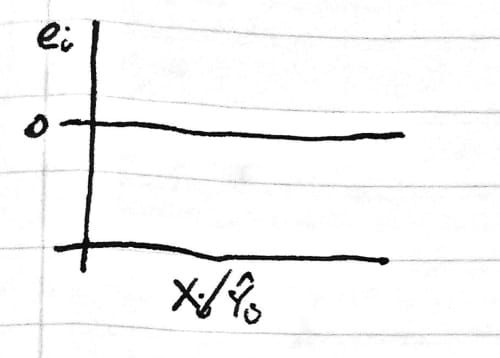
\includegraphics[width=.9\linewidth]{./images/empty_res-1.jpg}
\caption{\label{fig:org63ff33a}Empty Residual Plot}
\end{figure}

\begin{enumerate}
\item Tests
\label{sec:orgd7e1fdf}
\begin{enumerate}
\item Non-linearity of regression function
A pattern indicates linear regression not appropriate
\end{enumerate}

\begin{figure}[htbp]
\centering
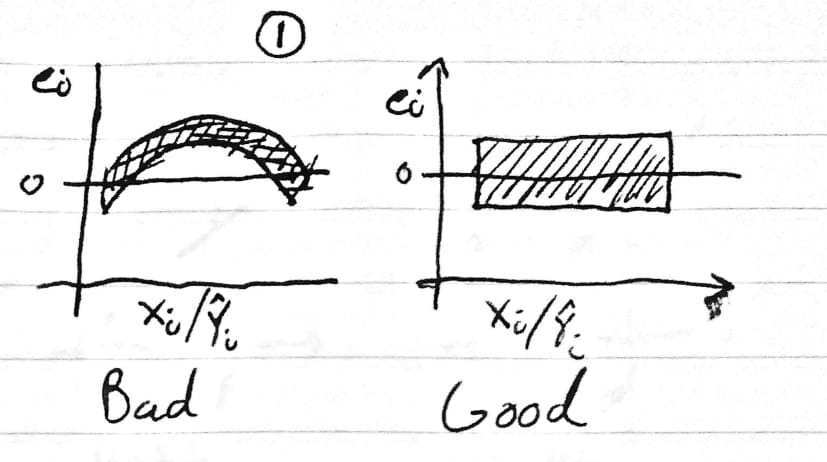
\includegraphics[width=.9\linewidth]{./images/resplot_1-1.jpg}
\caption{\label{fig:org4843ac6}Plots 1}
\end{figure}
\begin{enumerate}
\item Non-constancy of error terms
Fanning indicates different variances for different values of \(X_i or \hat{Y_i}\)

\begin{figure}[htbp]
\centering
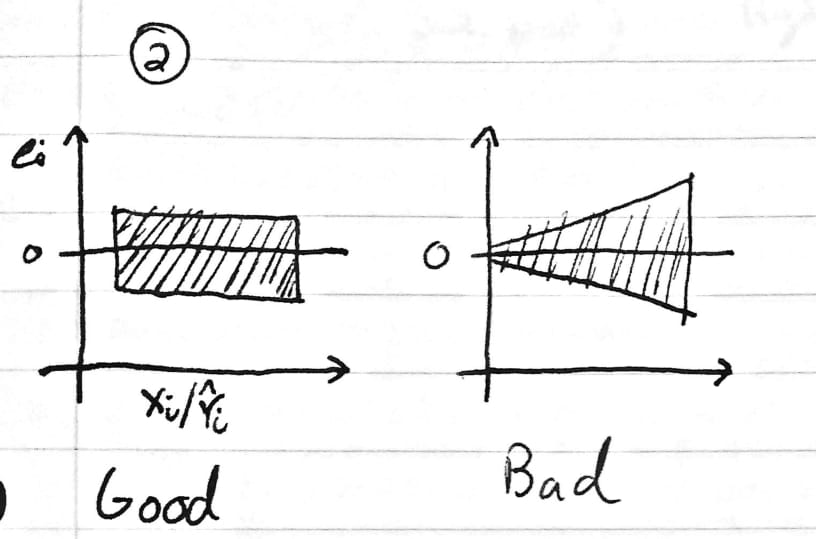
\includegraphics[width=.9\linewidth]{./images/resplot_2-1.jpg}
\caption{\label{fig:orgb511b12}Plots 2}
\end{figure}
\item Presence of outliers
Graph Semi-studentized residuals on a Residual plot \textbf{OR} a Box Plot

\begin{figure}[htbp]
\centering
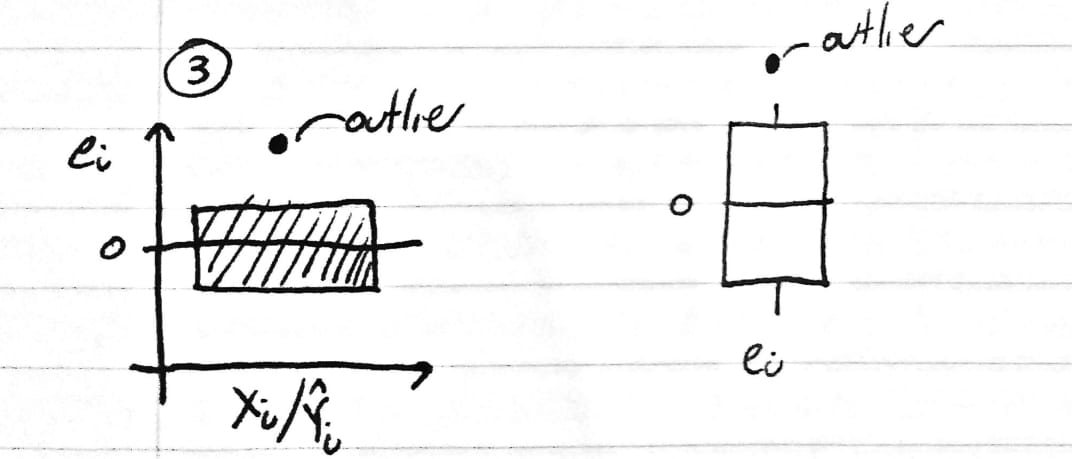
\includegraphics[width=.9\linewidth]{./images/resplot_3-1.jpg}
\caption{\label{fig:org6e32aaf}Plots 3}
\end{figure}
if \(|e_i^*| \geq 4\), outlier
\item Non-independence of error terms (more of a concern with time-series)
No pattern is good. Error terms safe to assume independent.

\begin{figure}[htbp]
\centering
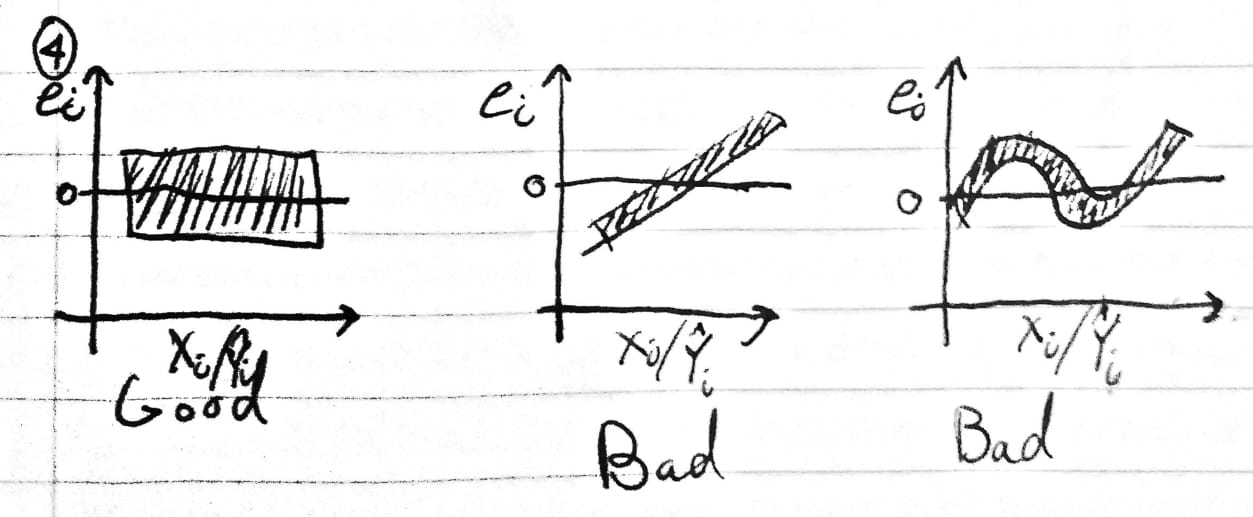
\includegraphics[width=.9\linewidth]{./images/resplot_4-1.jpg}
\caption{\label{fig:orgb0c893e}Plots 4}
\end{figure}
\item Normality of Error Terms
\begin{itemize}
\item Use a normal probability plot. The closer the points the fall on a straight
line, the closer they are to a normal distribution.

\begin{figure}[htbp]
\centering
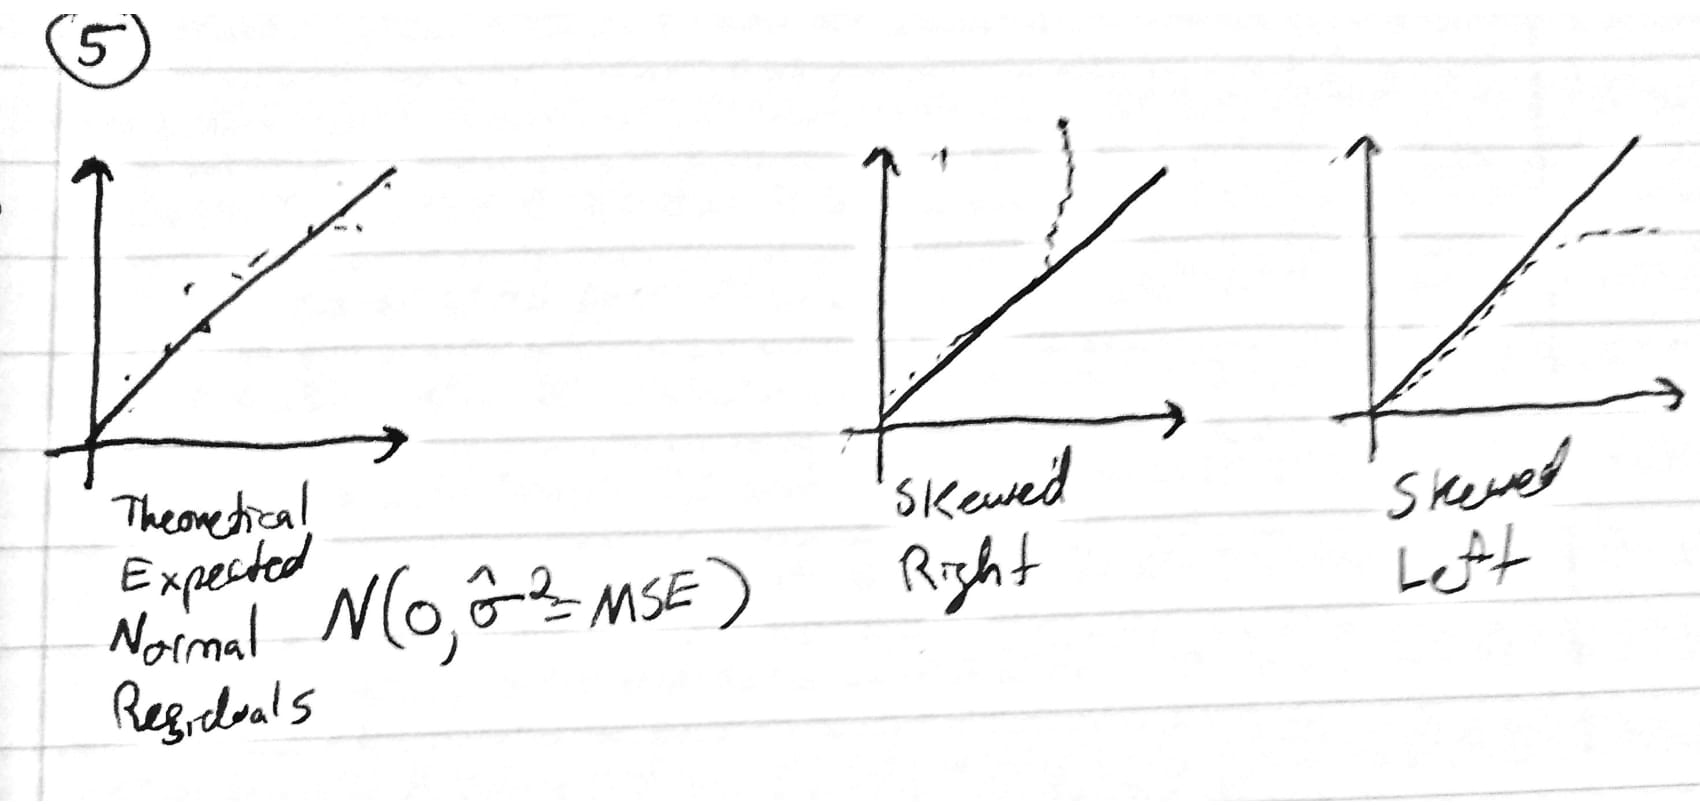
\includegraphics[width=.9\linewidth]{./images/resplot_5-1.jpg}
\caption{\label{fig:org1dc56fb}Plots 5}
\end{figure}
\end{itemize}
\item Omission of Important Predictors?
A Pattern indicates that there might be a relationship between the residuals
and some other predictor. This can be used to determine whether a predictor
should be used \uline{before} modeling it. Probably not as necessary anymore since
it is easy to run and compare models.
\end{enumerate}
\end{enumerate}
\subsubsection{Test of Randomness}
\label{sec:org1267220}
\begin{enumerate}
\item Durbin-Watson Test
\label{sec:org9a85169}

\begin{equation}
\begin{split}
H_0: \phi = 0 & \text{where $\phi$ is an autocorrelation coefficient} \\
H_A: \phi > 0 & \text{most assume positive correlation}
\end{split}
\end{equation}

\begin{verbatim}
lmtest::dwtest(modle)
\end{verbatim}
\item Shapiro-Wilk Test for Normality
\label{sec:orgd5f4bb0}
Not writing much here because I know it already
\begin{verbatim}
shapiro.test()
\end{verbatim}
\end{enumerate}
\subsubsection{Constant Variance}
\label{sec:orgaed6f73}
\begin{enumerate}
\item Brown-Forsyth Test
\label{sec:orgdee7802}
Robust since it uses Median
\begin{verbatim}
lawstat::levene.test()
\end{verbatim}
\item Breusch-Pagan Test
\label{sec:org400c909}
Sensitive to departures from Normality

\(log(\sigma^2) = \gamma_0 + \gamma_1 x_i\)

\begin{equation}
\begin{split}
H_0: \gamma_1 = 0\\
H_A: \gamma_1 \neq 0
\end{split}
\end{equation}

\begin{verbatim}
lmtest::bptest()
\end{verbatim}

\textbf{NOTES}: Heteroscedascity means non-constant variance
\end{enumerate}
\section{Session 4 - Transformations \& Inference (2019/10/02)}
\label{sec:org96408b7}
\subsection{Transformations}
\label{sec:org9381a74}
If non-normality and unequal error variance:
\begin{enumerate}
\item Transform Y: \(Y' = f(Y)\)
\item Transform X: \(X' = f(X)\)
\end{enumerate}

If non-linearity (rarer)
\begin{enumerate}
\item Transform X: \(X' = f(X)\)
\end{enumerate}

In order to determine which transformation to choose, look at the raw data and
make a judgement call.

\uline{In Class Example}

\(Y_i' = log(Y_i) = \beta_0 + \beta_1 X_i + \epsilon_i \equiv Y_i = exp(\beta_0 +
\beta_1 X_i + \epsilon_)i\)

A 1 unit increase in X is associated with a \(exp(\beta_1)\) multiplicative effect
on the \textbf{geometric} mean. This \href{https://stats.idre.ucla.edu/other/mult-pkg/faq/general/faqhow-do-i-interpret-a-regression-model-when-some-variables-are-log-transformed/}{link} explains in detail the impact of log
transformed variables.

Geometric mean = \((\Pi x_i)^\frac{1}{n}\)

\(\hat{Y_i} = log(Y)\)

\(X_i' = \sqrt{x}\)

\(\hat{Y_i} = 4.896 + 4.325 X_i' \to exp(4.235) = 75.528\)

For each 1 unit increase in \(X'\), the estimated increase in the geometric mean
price is 75.53 times its previous value.

\subsubsection{Box-Cox Transformations}
\label{sec:org23410fa}
There is a value \(\lambda\) that is the optimal transformation to the response
for equal variance and normality. It is optimal in the sense that it finds the
value of \(\lambda\) which produces the smallest SSE for \(Y_i\).

\(Y_i^{\lambda} = \beta_0 + \beta_1 X_i + \epsilon_i \text{where} i \sim
\text{iid } N(0,
\sigma^2)\)

\begin{center}
\begin{tabular}{lrrrrr}
\(\lambda\) & 2 & 0.5 & 0 & -0.5 & -1\\
\hline
\(Y' = Y^{\lambda}\) & \(Y^2\) & \(\sqrt{Y}\) & log(Y) & \(\frac{1}{\sqrt{Y}}\) & \(\frac{1}{Y}\)\\
\end{tabular}
\end{center}

\begin{verbatim}
lindia::gg-boxcox(model)
\end{verbatim}

\subsection{Simultaneous Inference}
\label{sec:orgb8289b6}
\textbf{Goal}: Try to estimate more than one mean response at a time.

\((0.95)^3 = 0.857375\)

\subsubsection{Working-Hotelling Procedure}
\label{sec:org128482e}
Based on the confidence band for the regression line.

100(1 - \(\alpha\))\% simultanous confidence limits for g mean responses \(E(Y_h)\)

\(Y_h \pm W \sqrt{MSE(\frac{1}{n} +\frac{(X_h - \bar{X})^2}{\Sigma(X_i - \bar{X})^2})} \text{where } W^2 = 2 F_{1- \alpha, 2, n - 2}\)

\begin{verbatim}
qf(1 - $\alpha$, 2, n - 2)
\end{verbatim}

\subsubsection{Bonferonni Procedure}
\label{sec:org03325bb}

\(Y_h \pm B \sqrt{MSE(\frac{1}{n} + \frac{(X_h - \bar{X})^2}{\Sigma(X_i - \bar{X})^2}
)} \text{where } B = t_{1 -\frac{\alpha}{2g}, n - 2}\)

\begin{verbatim}
qt(1 - alpha / 2g, n - 2)
\end{verbatim}
\section{Session 5 - Prediction \& Linear Algebra in Regression}
\label{sec:org42ab00b}
\subsection{Simultaneous Intervals}
\label{sec:org517068e}
\subsubsection{Confidence}
\label{sec:orgc7125a6}
Using the Bonferonni adjustment, The simultanous confidence interval for mean winning percentage for RunDiff of
\(X_h = -100,0,100\) has a confidence level = \(1 - \frac{\alpha}{g}\) where \(\alpha
= .05\) and \(g = 3\)

This is good for a smaller number of predictors. i.e. \(g < 10\)
\subsubsection{Prediction}
\label{sec:org0c9d8bb}
\textbf{Bonferroni}: \(\hat{Y_h} \pm t_{1 -\frac{\alpha}{2g}, n-2}
\sqrt{\text{MSE}(1 + \frac{1}{n} +\frac{(x_h - \bar{x})^2}{\Sigma(x_i - \bar{x})^2})}\)
level = \(1 - \frac{\alpha}{g}\)

\textbf{Scheffe}: \(\hat{Y_h} \pm S \sqrt{\text{MSE}(1 + \frac{1}{n} +\frac{(x_h -
 \bar{x})^2}{\Sigma(x_i - \bar{x})^2})}\) where \(S = \sqrt{g F_{1 - \alpha,g,n-2}}\)

Scheffe is more efficient with a larger \textbf{g} (i.e. g > 10). An in-class example
showed that this was not the case so the jury is still out.
\subsection{Inverse Prediction (``Calibration'')}
\label{sec:org294d8c2}

First, construct a model where \(Y = X\)

\uline{Goal}: Make a prediction of X that was used to predict a new value of Y.

\begin{equation}
\begin{split}
\hat{Y_i} & = \beta_0 + \beta_1 X_i + \epsilon_i \text{ where } \epsilon_i \sim \text{ iid } N(0, \sigma^2)\\
\hat{Y} & = b_0 + b_1 x
\end{split}
\end{equation}

We are given \(Y_{h(new)}\), so what is \(X_{h(new)}\)?

\(\hat{X_h(new)} = \frac{Y_{h(new)} - b_0}{b_1}\)

\(\hat{X_{h(new)}} \pm t_{1 - \frac{\alpha}{2},n-2} \sqrt{\frac{MSE}{b_1^2} (1 + \frac{1}{n} +\frac{(x_{h(new)} - \bar{x})^2}{\Sigma(x_i - \bar{x})^2})}\)

\begin{verbatim}
investr::calibrate(model, Y, interval = "Wald")
\end{verbatim}

The approximate confidence interval is appropriate if the following quantity is
small (i.e. < .1):

\(\frac{t_{1 - \frac{\alpha}{2}, n - 2}^2 MSE}{b_1^2 \Sigma (X_i - \bar{X})^2}\)

\subsection{Linear Algebra in Regression}
\label{sec:org4e98a85}
\subsubsection{Review}
\label{sec:org9742f01}

\(\underset{(n X 1)}{\vec{Y}} =
\begin{bmatrix}
Y_1\\
Y_2\\
...\\
Y_n
\end{bmatrix}\)

\(\underset{(1 \times n)}{\vec{Y^T}} = \begin{bmatrix}
Y_1 & ... & Y_n
\end{bmatrix}\)

\textbf{Design Matrix}

\(\underset{(n \times 2)}{X} = \begin{bmatrix}
1 & x_1\\
1 & x_2\\
... & ...\\
1 & x_n
\end{bmatrix}\)

\(\underset{(2 \times n)}{x^T} = \begin{bmatrix}
1 & ... & 1\\
x_1 & ... & x_n
\end{bmatrix}\)

\begin{enumerate}
\item Matrix Addition \& Subtraction
\label{sec:orged16da0}
\begin{equation}
\begin{split}
Y_i = & E(Y_i) + \epsilon_i\\
\vec{Y} = & E(\vec{Y}) + \vec{\epsilon}\\
E(\vec{Y}) = & \begin{bmatrix}
E(Y_1)\\
...\\
E(Y_n)
\end{bmatrix}\\
\vec{\epsilon{}} = & \begin{bmatrix}
\epsilon_1\\
...\\
\epsilon_n
\end{bmatrix}
\end{split}
\end{equation}

\item Matrix Multiplication
\label{sec:orga3fc4b3}
\begin{equation}
\begin{split}
\underset{(1 \times n)(n \times 1)}{\vec{Y}^T \vec{Y}} = & \begin{bmatrix}
Y_1 & ... & Y_n
\end{bmatrix}\begin{bmatrix}
Y_1\\
...\\
Y_n
\end{bmatrix} = \sum_{1}^{n}Y_i^2\\
\underset{(2 \times n)(n \times 2)}{X^T X} = & \begin{bmatrix}
1 & ... & 1\\
x_1 & ... & x_n
\end{bmatrix} \begin{bmatrix}
1 & x_1\\
... & ...\\
1 & x_n
\end{bmatrix} = \begin{bmatrix}
n & \Sigma X_i\\
\Sigma X_i & \Sigma X_i^2
\end{bmatrix}\\
\underset{(2 \times n)(n \times 1)}{X^T \vec{Y}} = & \begin{bmatrix}
1 & ... & 1\\
x_1 & ... & x_n
\end{bmatrix} \begin{bmatrix}
Y_1\\
...\\
Y_n
\end{bmatrix} = \begin{bmatrix}
\Sigma Y_i\\
\Sigma X_iY_i
\end{bmatrix}
\end{split}
\end{equation}
\item Special Matrices
\label{sec:orgd3cf42f}
\textbf{Symmetric}: \(A = A^T\)
This implies a square matrix. i.e. n x n

\textbf{Diagonal}: \(\underset{(n \times n)}A = \begin{bmatrix}
a_{11} & 0 & ... & 0\\
0 & a_{22} & ... & 0\\
... & ... & ... & ...\\
0 & 0 & 0 & a_{nn}
\end{bmatrix}\)

\textbf{Identity Matrix}: \(\underset{(n \times n)}I = \begin{bmatrix}
1 & ... & 0\\
... & 1 & ...\\
0 & ... & 1
\end{bmatrix}\)

\textbf{Scalar}: \(gI = \begin{bmatrix}
g & ... & 0\\
... & g & ...\\
0 & ... & g
\end{bmatrix}\) where \(g\) is a scalar value


\textbf{One vectors}
\begin{equation}
\begin{split}
\underset{(n \times 1)}{\vec{1}} = & \begin{bmatrix}
1\\
...\\
1
\end{bmatrix}\\
\underset{(n \times n)} J = & \begin{bmatrix}
1 & ... & 1\\
... & 1 & ...\\
1 & ... & 1
\end{bmatrix}\\
\underset{(1 \times n)(n \times 1)}{\vec{1}^T \vec{1}} = & n\\
\underset{(n \times 1)(1 \times n)}{\vec{1} \vec{1}^T} = & \begin{bmatrix}
1\\
...\\
1
\end{bmatrix} \begin{bmatrix}
1 & ... & 1
\end{bmatrix} = J
\end{split}
\end{equation}

\item Inverse of a Matrix
\label{sec:orgc5db48d}
\begin{equation}
\begin{split}
\underset{(2 \times 2)}{A} = &\begin{bmatrix}
a & b\\
c & d
\end{bmatrix}\\
\underset{(2 \times 2)}{A^-1} = & \frac{1}{det(A)} \begin{bmatrix}
d & -b\\
-c & a
\end{bmatrix} = \frac{1}{ad - bc} \begin{bmatrix}
d & -b\\
-c & a
\end{bmatrix}
\end{split}
\end{equation}

\textbf{Application to Regression}

\begin{equation}
\begin{split}
\underset{2 \times 2}{(X^T X)^-1} = & \frac{1}{det(X^T X)} \begin{bmatrix}
\Sigma x_i^2 & - \Sigma x_i\\
- \Sigma x_i & n
\end{bmatrix} = ... = \begin{bmatrix}
\frac{\Sigma x_i^2}{n \Sigma (x_i - \bar{x})^2} & - \frac{\Sigma x_i}{n \Sigma (x_i - \bar{x})^2}\\
- \frac{\Sigma x_i}{n \Sigma (x_i - \bar{x})^2} & \frac{n}{n \Sigma (x_i - \bar{x})^2}
\end{bmatrix}\\
det(X^T X) = & n \Sigma x_i^2 - (\Sigma x_i)^2\\
& = n \Sigma x_i^2 - \frac{n (\Sigma x_i)^2}{n^2}\\
& = n [ \Sigma x_i^2 - \frac{(\Sigma x_i)^2}{n}]\\
& = n \Sigma (x_i - \bar{x})^2
\end{split}
\end{equation}

\textbf{Side Note}

\begin{equation}
\begin{split}
\Sigma x_i = & n \bar{x}\\
\Sigma (x_i - \bar{x})^2 = & \Sigma x_i^2 - n \bar{x}^2\\
\Sigma x_i^2 = & \Sigma (x_i - \bar{x})^2 + n \bar{x}^2\\
(X^T X)^-1 = & \begin{bmatrix}
\frac{1}{n} + \frac{\bar{x}^2}{\Sigma (x_i - \bar{x})^2} & - \frac{\bar{x}}{\Sigma (x_i - \bar{x})^2}\\
- \frac{\bar{x}}{\Sigma (x_i - \bar{x})^2} & \frac{1}{\Sigma (x_i - \bar{x})^2}
\end{bmatrix}
\end{split}
\end{equation}
\item Matrix Rules
\label{sec:orgd68dbfc}
\begin{equation}
\begin{split}
A + B = & B + A\\
(A + B) + C = & A + (B + C)\\
(AB)C = & A(BC)\\
C(A + B) = & CA + CB\\
\\
(A^T)^T = & A\\
(A + B)^T = & A^T + B^T\\
(AB)^T = & B^T A^T\\
\\
(AB)^{-1} = & B^{-1} A^{-1}\\
(A^-1)^{-1} = & A\\
(A^T)^{-1} = & (A^{-1})^T
\end{split}
\end{equation}
\end{enumerate}

\subsubsection{Expectations}
\label{sec:orgd10446d}
\begin{equation}
\begin{split}
\underset{(n \times 1)}{\vec{Y}} = & \begin{bmatrix}
Y_1\\
...\\
Y_n
\end{bmatrix}\\
\underset{(n \times 1)}{E(\vec{Y})} = & \begin{bmatrix}
E(Y_1)\\
...\\
E(Y_n)
\end{bmatrix}\\
\vec{\epsilon} = & \begin{bmatrix}
\epsilon_1\\
...\\
\epsilon_n
\end{bmatrix}\\
E(\vec{\epsilon}) = & \vec{0}
\end{split}
\end{equation}

\subsubsection{Variance-Covariance Matrix}
\label{sec:org3d15192}

\begin{equation}
\begin{split}
\sigma^2(\vec{Y}) = & \begin{bmatrix}
Var(Y_i) & ... & Cov(Y_1, Y_n)\\
... & ... & ...\\
Cov(Y_n, Y_1) & ... & Var(Y_n)
\end{bmatrix}
\end{split}
\end{equation}

When \(Y_i\) independent, the off diagonals are 0 meaning \(\sigma^2(\vec{Y}) =
\sigma^2 I\)
\textbf{Aside}

\begin{equation}
\begin{split}
Var(Y) = & E[ (Y - E(Y))^2 ]\\
\sigma^2(\vec{Y}) = & E [ (\vec{Y} - E(\vec{Y}))(\vec{Y} - E(\vec{Y}))^T ]
\end{split}
\end{equation}

Let \(\underset{(p \times 1)}{\vec{W}} = \underset{(p \times n)(n \times 1)}{A
\vec{Y}}\) where A is a matrix of \textbf{constants} and Y is a \textbf{random vector}

\begin{equation}
\begin{split}
E(A) = & A\\
E(\vec{W}) = & AE(\vec{Y})\\
\sigma^2(\vec{W}) = & E[ (\vec{W} - E(\vec{W}))(\vec{W} - E(\vec{W}))^T ]\\
= & E[ (A \vec{Y} - AE(\vec{Y}))(A \vec{Y} - A E(\vec{Y}))^T ]\\
= & E[ A(\vec{Y} - E(\vec{Y}))(A(\vec{Y} - E(\vec{Y}))^T ]\\
= & E[ A(\vec{Y} - E(\vec{Y}))(\vec{Y} - E(\vec{Y}))^T A^T]\\
= & A E[ (\vec{Y} - E(\vec{Y}))(\vec{Y} - E(\vec{Y}))^T ] A^T\\
= & A \sigma^2(\vec{Y}) A^T
\end{split}
\end{equation}

\subsubsection{Multivariate Normal Distribution}
\label{sec:orgbc73895}
\begin{equation}
\begin{split}
\underset{(p \times 1)}{\vec{Y}} = & \begin{bmatrix}
Y_1\\
...\\
Y_p
\end{bmatrix}\\
\underset{(p \times 1)}{\vec{\mu}} = & \begin{bmatrix}
\mu_1\\
...\\
\mu_p
\end{bmatrix}
\end{split}
\end{equation}


\(\underset{(p \times p)}{\Sigma}\) = Variance-Covariance Matrix

\(f(\vec{Y}) = \frac{1}{(2 \pi )^{\frac{P}{2}}
\sqrt{det(\Sigma)}}exp(-\frac{1}{2}(\vec{Y} - \vec{\mu})^T \Sigma^{-1}
(\vec{Y} - \vec{\mu}))\)

If \(Y_1, ..., Y_p\) are jointly normally distributed (i.e in the multivariate
normal distr.), then \(Y_k \sim N(\mu_k, \sigma^2_k)\) where \(k = [1, p]\)

Recall the Linear Regression equation \(Y_i \beta_0 + \beta_1 X_i + \epsilon_i\)
where \(\epsilon_i \sim N(0, \sigma^2)\).

\(\underset{(n \times 1)}{\vec{Y}} = \underset{(n \times 2)(2 \times 1)}{X
\vec{\beta}} + \vec{\epsilon}\) where \(\underset{(n \times 1)}{\vec{\epsilon}}
\sim N_n(\vec{0}, \sigma^2 I)\)

\(N_n\) is a dimensions of a multivariate normal

\(\vec{\beta} = \begin{bmatrix}
\beta_0\\
\beta_1
\end{bmatrix}\)

\(E(\vec{Y}) = X \vec{\beta}\)

\subsubsection{Least Squares Estimation}
\label{sec:org1eecc2a}
\textbf{Normal Equations from Week 2}

\begin{equation}
\begin{split}
n b_o + b_1 \Sigma x_i = \Sigma Y_i\\
b_0 \Sigma X_i + b_1 \Sigma X_i^2 = \Sigma X_i Y_i
\end{split}
\end{equation}

\(X^T X \vec{b} = X^T \vec{Y}\)

So?

\textbf{Least Squares Estimator}: \(\vec{b} = (X^T X)^{-1} X^T \vec{Y}\)

\(\underset{(n \times 1)}{\vec{\hat{Y}}} = \underset{(n \times 2)(2 \times
1)}{X \vec{b}} = (X^T X)^{-1} X^T \vec{Y}\)

\begin{enumerate}
\item Hat Matrix
\label{sec:org6d76b91}
\(H = (X^T X)^{-1} X^T\)

The Hat Matrix is important for computing diagnostics for the model such as
Cook's Distance.

\textbf{Properties}
\begin{itemize}
\item symmetric (\(H^T = H\))
\item Idempotent (\(HH = H\))
\end{itemize}

\item Residuals
\label{sec:org66fcae4}
\(E_i = Y_i - \hat{Y_i} \to \vec{Y} - \vec{\hat{Y}} = \vec{Y} - X \vec{b} =
\vec{Y} - H \vec{Y} = (I - H) \vec{Y}\)

\(\sigma^2(\vec{e}) = \sigma^2(I - H)\)

This is estimated by: \(MSE (I - H)\)
\end{enumerate}
\section{Session 6 - Sums of Squares and Multiple Linear Regression}
\label{sec:org6687ba9}

\subsection{Sum of Squares}
\label{sec:orgc2cbfd5}

\begin{equation}
\begin{split}
\underset{(1 \times n)(n \times 1)}{\vec{Y}^T \vec{Y}} = \Sigma Y_i^2
\end{split}
\end{equation}

\textbf{Quadratic Form}: Contains squares of observations \textbf{and} their cross products.
 These are known as second-degree polynomials.

Quadratic forms scaled by \(\sigma^2\) allow us to treat the random variable Y as
an observation of \(\chi^2_{n - 1}\) distribution.

This is unlike \(\sigma^2 (A \vec{Y}) = A \sigma^2 (\vec{Y}) A^T\) since that is
squaring a matrix of \textbf{constants} whereas \(\vec{Y}^T \vec{Y}\) squares a matrix
of \textbf{random variables} i.e. Y

\subsubsection{SSE}
\label{sec:orgd82aa1c}
\begin{equation}
  \begin{split}
   SSE = & \Sigma e_i^2\\
       = & \vec{e}^T \vec{e}\\
       = & \vec{Y}^T (I - H) \vec{Y}
  \end{split}
\end{equation}

\subsubsection{SSTo}
\label{sec:orgcabb49a}

\begin{equation}
  \begin{split}
    SSTo = & \Sigma (Y_i - \bar{Y})^2\\
         = & \Sigma Y_i^2 - \frac{(\Sigma Y_i)^2}{n}\\
         = & \vec{Y}^T (I - \frac{1}{n} J) \vec{Y}
  \end{split}
\end{equation}

\subsubsection{SSR}
\label{sec:org7f4f982}

\begin{equation}
  \begin{split}
    SSR = & \Sigma (\hat{Y_i} - \bar{Y})^2\\
        = & \vec{Y}^T (H - \frac{1}{n} J) \vec{Y}
  \end{split}
\end{equation}

\subsection{Mean Estimates \(\sigma^2\)}
\label{sec:orgfea7290}
\subsubsection{Mean Responses}
\label{sec:orgf11a509}
\(\hat{Y_h} = b_0 + b_1 X_h\)

so? we would like
\begin{equation}
\begin{split}
\underset{(1 \times 1)}{\hat{Y_h}} = \begin{bmatrix}
1 & X_h
\end{bmatrix}
\vec{b}
\end{split}
\end{equation}


Let \(\vec{X_h} = \begin{bmatrix}
1\\
X_h
\end{bmatrix}\)

Then, \(\hat{Y_h} = \vec{X_h}^T \vec{b}\)

This is an estimate of the mean response!
\subsection{Variance of \(\hat{Y_h}\)}
\label{sec:orgf3d23de}
\begin{equation}
  \begin{split}
    \underset{(1 \times 1)}{Var(\hat{Y_h})} = & Var(\vec{X_h}^T \vec{b})\\
                                            = & \vec{X_h}^T Var(\vec{b}) \vec{X_h}\\
                                            = & \vec{X_h}^T \sigma^2(X^T X)^{-1} \vec{X_h}\\
                                            = & \underset{(1 \times 2)(2 \times 2)(2 \times 1)}{\sigma^2 X_h^T (X^T X)^{-1} \vec{X_h}}
  \end{split}
\end{equation}
\subsection{Multiple Regression Models}
\label{sec:org80cce7c}

\(Y_i = \beta_0 + \beta_1 X_{i1} + ... + \beta_{p - 1} X_{i, p - 1} + \epsilon_i\)
where \(\epsilon_i \sim iid N(0, \sigma^2)\)

\(E(Y_i) = \beta_0 + \beta_1 X_{i1} + ... + \beta_{p - 1} X_{i, p - 1}\)

\(Y_i \sim indep N(E(Y_i), \sigma^2)\).

The parameters of this model are \{\(\beta\)\textsubscript{0}, \ldots{}, \(\beta\)\textsubscript{p}\}. Thus there are \textbf{p}
regression coefficients.

\subsubsection{Interpretation}
\label{sec:org4d767e9}
Using the model, \(Y_i = \beta_0 + \beta_1 X_{i,1} + \beta_2 X_{i,2}\)

let's interpret the coefficients.

\(\beta_0\): The mean response of Y when \(X_1 = 0, X_2 = 0\)

\(\beta_1\): For a fixed value of \(X_2\), the associated increase in mean response
in Y is \(\beta_1\) for every 1 unit increase in \(X_1\). \textbf{This is known as a
partial effect}

\(\beta_2\): For a fixed value of \(X_1\), the associated increase in mean response
in Y is \(\beta_2\) for every 1 unit increase in \(X_2\).

\(\beta_k\): Associated change in mean response of Y for every 1 unit increase in
\(X_k\), given all other predictors are held constant.

\subsubsection{Aside: Multi-Collinearity}
\label{sec:orgc9abeea}
\textbf{Multicollinearity} occurs when two or more predictors are highly correlated.
\begin{itemize}
\item Standard Errors blow up which makes test statistic small, which makes p-values
high. This affects the ability for us to make \textbf{inferences}
\item Multicollinearity is acceptable when using models for \textbf{prediction} but not
when using them for \textbf{inference}.
\end{itemize}
\subsubsection{Matrix Notation}
\label{sec:orgebefd7b}
\begin{equation}
  \begin{split}
    \underset{(n \times 1)}{\vec{Y}} = & \underset{(n \times p)(p \times 1)}{X \vec{\beta}} + \underset{(n \times 1)}{\vec{\epsilon}}\\
    \underset{(n \times n)}{Var(\vec{\epsilon})} = & \sigma^2 I
  \end{split}
\end{equation}
\begin{enumerate}
\item Fitted Values
\label{sec:org1ec9f36}
\(\hat{Y_i} = b_0 + b_1 X_{i,1} + ... + b_{p - 1} X_{i, p - 1}\)

\textbf{Residuals}: \(e_i = Y_i - \hat{Y_i}\)

\item Least Squares Estimators
\label{sec:org1c4ad6c}

\(\underset{(p \times 1)}{\vec{b}} = \underset{(p \times n)(n \times p)}{(X^T X)^{-1}} \underset{(p \times n)(n \times 1)}{X^T \vec{Y}}\)
\end{enumerate}
\subsubsection{ANOVA Table}
\label{sec:orgc323a9d}

\begin{center}
\begin{tabular}{llllll}
Source & SS & DF & MS & F & p-value\\
\hline
Regression & SSR = \(\Sigma (\hat{Y_i} - \bar{Y})^2\) & p - 1 & \(MSR = \frac{SSR}{p - 1}\) & \(F^* = \frac{MSR}{MSE}\) & \(P(F_{p-1, n-p} \geq F^*)\)\\
Error & SSE = \(\Sigma (Y_i - \hat{Y_i})^2\) & n - p & \(MSE = \frac{SSE}{n - p}\) &  & \\
Total & SSto = \(\Sigma (Y_i - \bar{Y})^2\) & n - 1 &  &  & \\
\end{tabular}
\end{center}

\subsubsection{Omnibus F-Test for Regression Relation}
\label{sec:org8d1f275}
\begin{equation}
  \begin{split}
    H_0: \beta_1 = \beta_2 = ... = \beta_p = 0\\
    H_A: \text{ at least one } \beta_k \neq 0
  \end{split}
\end{equation}

Test statistic: \(F^* = \frac{MSR}{MSE}\).
If \(H_0\) is true, \(F^* \sim F_{p - 1, n - p}\)
\subsubsection{Coefficient of Multiple Determination}
\label{sec:org1d8f7cb}
\(R^2 = 1 - \frac{SSE}{SSTo}\)

The issue with \(R^2\) is that it increases with the number of predictors
\textbf{irrespective} of the predictor improving the model.

\(R_{adj}^2 = 1 - \frac{\frac{SSE}{n - p}}{\frac{SSTo}{n - 1}}\)
\subsubsection{Coefficient of Multiple Correlation}
\label{sec:org8aafc1a}

\(R = \sqrt{R^2}\)

\subsubsection{Inferences in \(\beta_k\)}
\label{sec:org79079a3}
\begin{equation}
  \begin{split}
    H_0: \beta_k = 0\\
    H_A: \beta_k \neq 0
  \end{split}
\end{equation}

\textbf{Test Statistic}: \(t^* = \frac{b_k}{SE_{bk}}\)

If \(H_0\) is true, then \(t^* \sim t_{n - p}\)

p-value = \(2 P(t_{n - p} \geq |t|)\)

\begin{verbatim}
2 * (1 - pt(abs(t.star), n - p))
\end{verbatim}

\(100(1 - \alpha)%\) C.I. for \(\beta_k\): \(b_k \pm t_{1 - \frac{\alpha}{2}, n - p}
SE_{bk}\)

\section{Session 7 - Multiple Regression \& Qualitative$\backslash$/Quantitative Predictors}
\label{sec:org1a3634f}
\subsection{Multiple Regression}
\label{sec:org0709912}

\subsubsection{Extra Sums of Squares}
\label{sec:org46070b8}
\textbf{Def}: The marginal reduction in SSE when one or several predictors are added to
the regression model, \textbf{given} other predictors are already in the model.

\(SSR(X_2 | X_1) = & SSE(X_1) - SSE(X_1, X_2)\\
  SSR(X_2 | X_1) = & SSR(X_1, X_2) - SSR(X_1)\)

These are equivalent because any reduction in SSE implies an increase in SSR per
the ANOVA definition: \(SSTo = SSR + SSE\)

\begin{enumerate}
\item Multiple Predictors
\label{sec:org51584de}

\(SSR(X_3 | X_1, X_2) = & SSE(X_1, X_2) - SSE(X_1, X_2, X_3)\\
SSR(X_3 | X_1, X_2) = & SSR(X_1, X_2, X_3) - SSR(X_1, X_2)\)

\(SSR(X_1, X_2) = SSR(X_2) + SSR(X_1 | X_2)\)

\begin{center}
\begin{tabular}{llrl}
Source & SS & df & MSE\\
\hline
Regression & \(SSR(X_1, X_2, X_3)\) & 3 & \(MSR(X_1, X_2, X_3)\)\\
\(X_1\) & \(SSR(X_1)\) & 1 & \(MSR(X_1)\)\\
\(X_2 \vert X_1\) & \(SSR(X_2 \vert X_1)\) & 1 & \(MSR(X_2 \vert X_3)\)\\
\(X_3 \vert X_1, X_2\) & \(SSR(X_3 \vert X_1, X_2)\) & 1 & \(MSR(X_3 \vert X_1, X_2\))\$\\
Error & \(SSE(X_1, X_2, X_3)\) & n - 4 & \(MSE(X_1, X_2, X_3)\)\\
Total & SSTo & n - 1 & \\
\end{tabular}
\end{center}

\item Hypothesis Test - \(\beta_k = 0\)
\label{sec:org21e4ee6}
\(H_0: \mu_k = 0\\
H_A: \mu_k \neq 0\)

This is the \(\mu_k X_k\) dropped from the model.

\textbf{Test Statistic}: \(t^* = \frac{b_k}{SE_{bk}}\) \(df = n - p\)

\begin{enumerate}
\item Full model
\label{sec:orgc020306}
\(Y_i = \mu_0 + \mu_1 X_1 + ... + \mu_{p - 1} X_{i, p-1} + \epsilon_i\)

``p - 1'' predictor variables

\(SSE(F) = SSE(X, ..., X_{p - 1})\)

\item Reduced Model
\label{sec:org5f19d6c}
\(Y_i = \mu_0 + \mu_1 X_1 + ... + \mu_{p - 2} X_{i, p - 2} + \epsilon_i\)


``p - 2'' predictor variables

\(SSE(R) = SSR(X, ..., X_{k - 1}, X_{p - 1})\)

\(F^* = SSE(R) - SSE(F) = \frac{df_R - df_F}{\frac{SSE(F)}{df_F}} = \frac{
\frac{SSE(X_1, ..., X_{k - 1}, X_k, ..., X_{p - 1}) - SSE(X, ..., X_{p -
1})}{n - (p - 1) - (n - p)}}{\frac{SSE(X, ..., X_{p - 1})}{n - p}}\)
\end{enumerate}


\item Hypothesis Test - \(\beta_0 = ... = \beta_k = 0\)
\label{sec:org37b3fbb}
\begin{enumerate}
\item Reduced Model
\label{sec:orgf640c3c}
\(Y_i = \mu_0 + \mu_1 X_{i1} + ... + \mu_{k - 1} X_{i,k - 1} + \mu_k X_{ik} + ... + \mu_{p - 1} X_{i, p - 1} + \epsilon_i\)

``p - g - 1'' predictors \textbf{OR} ``p - g'' regression coefficients

\(F^* = \frac{\frac{SSE(X_1, ..., X_{k - 1}, X_k, ..., X_{p - 1}) - SSE(X, ..., X_{p -
1})}{n - (p - g) - (n - p)}}{\frac{SSE(X, ..., X_{p - 1})}{n - p}} = \frac{SSR(X_k, ..., X_{k + (g - 1)} |
X_k, ..., X_{k + g}, ..., X_{p - 1})}{MSE(X_1, ..., X_{p - 1})}\)
If \(H_0\) is true, \(F^* \sim F_{g, n - p}\)
\end{enumerate}
\item \(R^2\)
\label{sec:org27215d4}
\(R^2\): Coefficient of multiple determination
\begin{itemize}
\item proportion of variation in Y explained by the regression of Y on \(X_1, ...,
  X_{p - 1}\)
\end{itemize}

\uline{Ex}

\(Y_i = \mu_0 + \mu_1 X_{i,1} + \mu_2 X_{i,2}\)

\(SSE(X_2)\): variation when only \(X_2\) is in the model.

\(SSE(X_1, X_2)\): variation when both \(X_1,X_2\) are in the model.

Marginal reduction in variation when X\textsubscript{1} is added to the model?

\(\frac{SSE(X_2) - SSE(X_1, X_2)}{SSE(X_2)}\)

\(R_{Y_1/Y_2}^2 = \frac{SSR(X_1 | X_2)}{SSE(X_2)}\)

\(R_{Y_2/Y_1}^2 = \frac{SSR(X_2 | X_1)}{SSE(X_1)}\)

3 predictors

\(R_{Y3|2,1}^2 = \frac{SSR(X_3 | X_1, X_2)}{SSE(X_1, X_2)}\)

Recipe for correlation coefficient:
\begin{enumerate}
\item Take sqrt of partial \(R^2\)
\item Sign of partial correlation = sign of correlation corresponding coefficient
\end{enumerate}
\end{enumerate}

\subsection{Multi-collinearity}
\label{sec:org7258e50}

Predictors that are highly correlated with each other. \textbf{10 N values per predictor}

\subsubsection{Effects}
\label{sec:org6f51ff8}
\begin{enumerate}
\item There is no unique sum of squares that can be assigned to the predictor
variable
\item May inflate standard error of \(b_k\) least square error.
\end{enumerate}

It does not greatly impact the value of predictions.

\({ETA}^2\) tells \(R^2\) given the previously given variable \(R^2\)
\subsection{Polynomial Regression Models}
\label{sec:orgc4c6ea3}

\begin{itemize}
\item true curvilinear response
\item true curvilinear response is unknown but a polynomial function provides a good
approximation to the true function.
\end{itemize}


One prediction variable \textbf{and} second order:

\(Y_i = \mu_0 + \mu_1 X + \mu_2 X^2 + \epsilon_i\) where \(X_i = x_i - \bar{x}\)

\(E(Y) = \mu_0 + \mu_1 X_1 + \mu_2 X^2\)

Two parameters \textbf{and} second order:

\(x_{i,1} = x_{i,1} - \bar{x_1}\)

\(X_{i,2} = x_{i,2} - \bar{x_2}\)

\(Y_i = \beta_0 \beta_1 X_{i,1} + \beta_2 X_{i,2} + \beta_3 X_{i,1}^2 + \beta_4
X_{i,2}^2 + \beta_5 X_{i,1} X_{i,2} + \epsilon_i\)

\uline{Strategy?} Fit higher order models and compare to reduced models.


\begin{verbatim}
summary(model)
\end{verbatim}

\(\hat{Y} =  b_0 + b_1 x + b_2 x^2\)
\(\hat{Y} =  b_0' + b_1' x + b_2' x^2\)

\(b_0' = b_0 - b_1 \bar{x} - b_2 \bar{x}^2\)

\(b_1' = b_1 - 2 b_2 \bar{x}\)

\(b_2' = b_2\)

Why do this? Solving a regression model with a non-linear \(E(Y_i)\)
\section{Session 8 - Interaction Models \& Model Selection}
\label{sec:orgdb781e0}
\subsection{Interaction Regression Models}
\label{sec:org5a9fbbf}
\begin{itemize}
\item p: \# of regression coefficients. i.e. parameters
\item p - 1: predictor variables
\end{itemize}

\subsubsection{Additive Effects}
\label{sec:orge8f9dbf}
\begin{equation}
\begin{split}
E(Y) = \sum_{i = 1}^{p - 1} f_K(x_k)
\end{split}
\end{equation}
\textbf{but} \(E(Y) = \beta_0 + \beta_1 X_1 + \beta_2 X_2 + \beta_3 X_1 X_2\) is \textbf{not}
 additive since \(X_1 X_2\) is an interaction term

Consider the following:

\(Y_i = \beta_0 + \beta_1 X_1 + \beta_2 X_2 + \beta_3 X_1 X_2 + \epsilon_i\) where
\(\epsilon_i \sim iid N(0, \sigma^2)\)

A one-unit \textbf{increase} in \(X_2\) for a fixed value of \(X_1\), results in an
associated change of \(\beta_1 + \beta_3 X_1\) units in mean response Y.

\begin{itemize}
\item \(\beta_3 = 0\) => additive model
\item \(\beta_3 > 0\) => reinforcement or synergistic interaction*
\item \(\beta_3 < 0\) => interference or antagonistic interaction*
\end{itemize}

*if \(\beta_1\) and \(\beta_2\) are negative, these terms flip

parallel lines indicate \textbf{additive} terms, otherwise \uline{interactive}

\textbf{Aside}
\begin{quote}
To avoid multicollinearity between predictors, center variables!
 \(X_{ik} = X_{ik} - \bar{X_k}\)

Does Standardizing also help reduce multicollinearity? Yes, but makes
interpretation more difficult. This is done in PCA and as I've seen,
interpreting PCA can be hairy or a best guess.
\end{quote}


\begin{itemize}
\item Try to identify possible interactions ahead of time prior to fitting the
model.
\item When looking at removing \textbf{one} term, the \(t\) statistic is sufficient to rule
out a parameter.
\end{itemize}

\subsubsection{Qualitative Predictors}
\label{sec:org58067a0}
Qualitative Predictor with two classes. i.e. two values
This is sometimes called: Indicators, Binary, dummy variables

For representing \(C\) classes, use \(C - 1\) indicator variables.

\uline{Example}

Let C = 4
\(C =\begin{bmatrix}
A\\
B\\
C\\
D
\end{bmatrix}\)

\begin{equation}
\begin{split}
Y_i = & \beta_0 + \beta_1 X_1 + \beta_2 X_2 \ \beta_3 X_3 + \beta_4 X_4 + \epsilon_i \text{ where }\\
X_2 = & \begin{cases}
1, &  A\\
0, & else
\end{cases}\\
X_3 = & \begin{cases}
1, &  B\\
0, & else
\end{cases}\\
X_4 = & \begin{cases}
1, &  C\\
0, & else
\end{cases}
\end{split}
\end{equation}

if \(X_2 = X_3 = X_4 = 0\), indicates effect of \(C = D\) on mean \(Y_i\)

\begin{equation}
\begin{split}
A: E(Y) = & (\beta_0 + \beta_2) + \beta_1 X_i\\
B: E(Y) = & (\beta_0 + \beta_3) + \beta_1 X_i\\
C: E(Y) = & (\beta_0 + \beta_4) + \beta_1 X_i\\
D: E(Y) = & (\beta_0) + \beta_1 X_i
\end{split}
\end{equation}

D is considered the \textbf{baseline category}

1 Qualitative variable and 1 Quantitative variable in the same model is known as
\textbf{ancova}: Analysis of Covariance. ANCOVA assumes that each group has the same slope.


\uline{Interpret \(\beta_0\)}: The diff in mean response of \(Y\) between \(A\) and \(D\)
group for a given value of \(X_1\)

\textbf{Estimate \(\beta_3 - \beta_4\)}
\begin{enumerate}
\item \(b_3 - b_4\)
\item \(Var(b_3 - b_4) = var(b_3) + var(b_4) - 2 cov(b_3, b_4)\)
\end{enumerate}

If doing time series, one can use indicator variables to model time periods

\subsection{Model and Variable Selection}
\label{sec:orgc47e2e4}
\subsubsection{Criterion for Model Selection}
\label{sec:orge7b7bf1}
p: \# of parameters (regression coefficients)

\begin{enumerate}
\item \(R^2_p\) or \(SSE_p\) criterion. Both indicate the same thing.

\(R_p^2 = 1 -\frac{SSE_p}{SSTo}\)

\textbf{Look for}
\begin{itemize}
\item \emph{High} \(R_p^2\)
\item \emph{Small} \(SSE_p\)
\end{itemize}

\item \(R_{a,p}^2\) or \(MSE_p\) criterion

\(R_p^2 = 1 -\frac{\frac{SSE_p}{n- p}}{\frac{SSTo}{n - 1}} = 1 -
   \frac{MSE_p}{\frac{SSTo}{n - 1}}\)

\textbf{Look For}:
\begin{itemize}
\item \emph{High} \(R_{a,p}^2\)
\item \emph{Small} \(MSE_p\)
\end{itemize}

\item Mallows' \(C_p\) Criterion

\(C_p = \frac{SSE_p}{MSE(X_1, ..., X_{p - 1})} - (n - 2p)\)

\(MSE(X_1, ..., X_{p - 1})\): MSE for the model with \textbf{all} potential predictors
of interest.

For largest possible value of \(P\), \(C_p = p\)

\uline{proof}
\end{enumerate}
\begin{equation}
\begin{split}
MSE = & \frac{SSE}{n - p}\\
\frac{SSE_p}{\frac{SSE_p}{n - p}} = & n - p - (n - 2p) =  p
\end{split}
\end{equation}

\textbf{Look for}
\begin{itemize}
\item \emph{Small} \(C_p\) \uline{or} \(C_P \leq p\). This means the model has a small amount of
bias.
\end{itemize}

Recall \(MSE(Y) = Bias^2(Y) + Var(Y)\)

\begin{enumerate}
\item \(AIC_p\) or \(SBC_p\) Criterion
\begin{itemize}
\item \(AIC_p\): Akaike's Information Criterion:  \(n ln(SSE_p) - n ln(n) + 2p\)
\begin{itemize}
\item \(-2 loglik + 2p\)
\end{itemize}
\item \(SBC_p\): Schwartz' Bayesian Information Criterion - \(n ln(SSE_p) - n
     ln(n) + p ln(n)\)
\begin{itemize}
\item \(-2 loglik + 2 ln(p)\)
\end{itemize}
\end{itemize}

\textbf{Look for}
\begin{itemize}
\item \emph{Small} \(SSE_p\)
\item \emph{Small} \(AIC_p\) and/or \(SBC_p\)
\end{itemize}

\item \(PRESS_p\) Criterion

Prediction Sum of Squares

\(PRESS_P = \sum_{1}^{n} (Y_i - \hat{Y_{i (i)}})^2\)

\textbf{\(\hat{Y_{i(i)}}\)}
\begin{enumerate}
\item Ignore the ith case
\item Fit model on remaining \(n - 1\) cases
\item Find Fitted value based on deleted ith case
\end{enumerate}

This is \textbf{not} the same as bootstrapping, mostly because there is no
resampling oging on.

\begin{verbatim}
   leaps::regsubsets(formula, data, method="exhaustive", nbest=30)
\end{verbatim}

\begin{verbatim}
   #+NAME: fortify_leaps
   fortify.regsubsets <- function(model, data, ...){
     require(plyr)
     stopifnot(model$intercept)
     models <- summary(model)$which
     rownames(models) <- NULL
     model_stats <- as.data.frame(summary(model)[c("bic","cp","rss","rsq","adjr2")])
     dfs <- lapply(coef(model, 1:nrow(models)), function(x) as.data.frame(t(x)))
     model_coefs <- plyr::rbind.fill(dfs)
     model_coefs[is.na(model_coefs)] <- 0
     model_stats <- cbind(model_stats, model_coefs)
     # terms_short <- abbreviate(colnames(models))
     terms_short <- colnames(models)
     model_stats$model_words <- aaply(models, 1, function(row) paste(terms_short[row], collapse = "+"))
     model_stats$size <- rowSums(summary(model)$which)
     model_stats
   }

   get_model_coefs <- function(model){
     models <- summary(model)$which
     dfs <- lapply(coef(model, 1:nrow(models)), function(x) as.data.frame(t(x)))
     model_coefs <- plyr::rbind.fill(dfs)
     model_coefs[is.na(model_coefs)] <- 0
     model_coefs
  }
\end{verbatim}
\end{enumerate}
\section{Session 9 - Model and Variable Selection \& Assessing Diagnostics}
\label{sec:org83e69b3}
\subsection{Model and Variable Selection}
\label{sec:orgc94f0b3}
\subsubsection{Automatic Search Procedures}
\label{sec:orgcf916f6}
\begin{enumerate}
\item Backward Selection
\label{sec:orgb3726f5}

Full Model -> reduce parameters to ``smallest'' AIC

\begin{verbatim}
step(model.full, direction = "backward")
\end{verbatim}

\item Forward Selection
\label{sec:orgd4d81c1}

Intercept-only model -> add parameters to ``smallest'' AIC

\begin{verbatim}
step(lm.null, scope = list(lower, upper), direction = "forward")
\end{verbatim}

\item Step-wise
\label{sec:org8662ba7}

Intercept-only model -> add one -> subtract$\backslash$/add one for ``smallest'' AIC

\begin{verbatim}
step(lm.null, scope = list(upper), direction = "both")
\end{verbatim}
\end{enumerate}

\subsubsection{Model Validation}
\label{sec:org72d0046}
\begin{enumerate}
\item Collect new data t ocheck the model and it's predictive validity

\(MSPR = \frac{\sum_{1}^{n^*} (Y_i - \hat{Y_i})^2}{n^*}\)

If MSPR approximately your Model's MSE, then your model is not necessarily
biased.
If the difference is large, MSPR is a good indicator on how well it predicts.

\textbf{Defintions}
\begin{itemize}
\item MSPR: Mean Square Prediction Error
\item \(Y_i\): Value of the response variable in the ith validation case
\item \(\hat{Y_i}\): Predicted value of the ith validation case using the model you
previously built.
\item \(n^*\): number of cases in the validation dataset.
\end{itemize}

\item Compare results with theoretical expectations empirical results, and
simulation results.
\item Use a holdout sample to check the model and its predictive ability. This is
standard practice for predictive models
\end{enumerate}

\subsection{Assessing Diagnostics}
\label{sec:orgbf3cfba}
\subsubsection{Added-variable Plots}
\label{sec:orgd910980}
Also known as:
\begin{itemize}
\item Partial Regression Plots
\item Adjusted Variable Plots
\end{itemize}

These plots show:
\begin{itemize}
\item Marginal Importance of this variable in reducing residual variability
\item May provide info about the nature of the marginal regression relation for
predictor variable \(X_k\) under consideration
\end{itemize}

\begin{enumerate}
\item Example
\label{sec:orgc99aea6}
\(Y_i = \beta_0 + \beta_1 X_{i1} + \beta_2 X_{i2} + \epsilon_i\)

\textbf{Goal}: What is \(X_i\)'s effect given that \(X_2\) is in the model?

\begin{equation}
\begin{split}
\hat{Y_i}(X_2) = b_0 + b_2 X_{i2}\\
e_i(Y | X_2) = Y_i - \hat{Y_i}(X_2)
\end{split}
\end{equation}

\emph{fitted values + residuals from the model with only \(X_2\)}

\begin{equation}
\begin{split}
\hat{X_{i1}}(X_2) = b_0^* + b_2^* X_{i2}\\
e_i(X_1 | X_2) = X_{i1} - \hat{X_i1} (X_2)
\end{split}
\end{equation}

\begin{quote}
fitted value + residuals from the model with \(X_1\) as the response and \(X_2\) as
the predictor.
\end{quote}

\item Reading Plots
\label{sec:org922c95f}

\begin{verbatim}
car::avPlots(model)
\end{verbatim}

\begin{figure}[htbp]
\centering
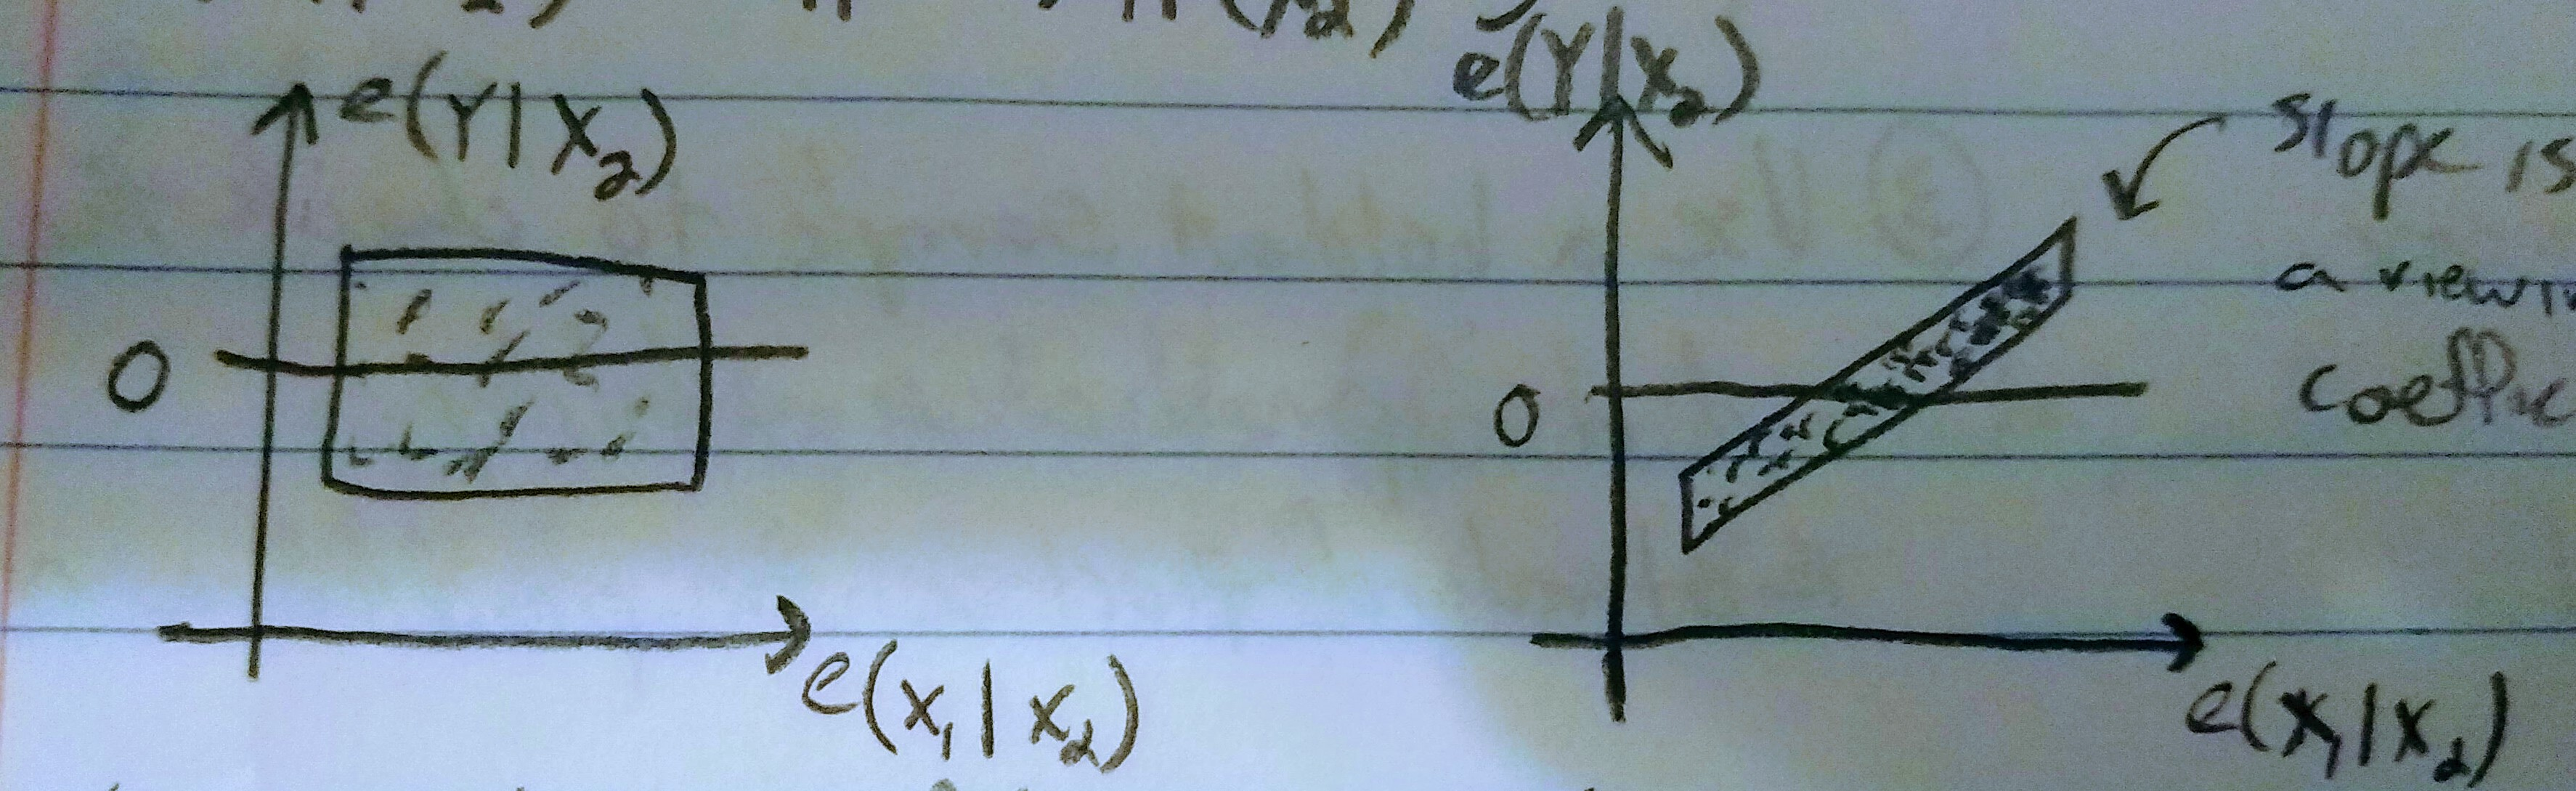
\includegraphics[width=.9\linewidth]{./images/avPlots.jpg}
\caption{\label{fig:orgcd5c716}Partial Residuals vs Fitted Values}
\end{figure}

\begin{enumerate}
\item Partial Residuals \(X_1\) vs Fitted Values

Notice the even distribution of residuals around y = 0. \(X_1\) provides no
useful information given \(X_2\) is in the model.

\item Partial Residuals \(X_2\) vs Fitted Values

Notice the pattern. \(X_1\) may be a good addition to the model given \(X_2\) is
already in the model.
\end{enumerate}

\textbf{Goal}: Identify outlying Y observations. i.e. which Y observations are
 influential on our own regression model?

\begin{itemize}
\item \uline{Residuals}: \(e_i = Y_i - \hat{Y_i}\)
\item \uline{Semi-studentized Residuals}: \(e^* = \frac{e_i}{\sqrt{MSE}}\)
\item \uline{Studentized Residuals}: \(R_i = \frac{e_i}{\sqrt{MSE(1 - h_{ii})}}\)

\(h_{ii}\): the ith diagonal value from the hat matrix H
\end{itemize}

\begin{verbatim}
rstandard(model)
\end{verbatim}
\end{enumerate}
\section{Session 10 - Outliers \& Weighted Least Squares}
\label{sec:org064afb4}
\subsection{Outliers}
\label{sec:org90963a5}
\subsubsection{Identifying Outlying Y Observations}
\label{sec:org5815a0a}
\begin{itemize}
\item Use Studentized Deleted Residuals to identify \emph{outlying Y Observations}
\end{itemize}

\textbf{Residuals}: \(e_i = Y_i - \hat{Y_i}\)

\textbf{Semi-studentized Residuals}: \(e_i^* = \frac{e_i}{\sqrt{MSE}}\)

\textbf{Studentized Residuals}: \(r_i =\frac{e_i}{\sqrt{MSE(1 - h_{ii})}}\)

\(h_{ii}\): Standard Error of \(e_i\). aka Standard Error of the ith residual

\textbf{Deleted Residuals}: \(d_i = Y_i - \hat{Y_{i(i)}} = \frac{e_i}{1 - h_{ii}}\)

\textbf{Studentized Deleted Residuals} (rstudent):

\begin{equation}
\begin{split}
t_i = & \frac{d_i}{SE_{d_i}}\\
= & \frac{e_i}{\sqrt{MSE_{(i)}(1 - h_{ii})}}\\
= & e_i \sqrt{\frac{n - p - 1}{SSE(1 - h_{ii}) - e_i^2} }
\end{split}
\end{equation}

\subsubsection{What is an Outling Y Observation?}
\label{sec:org5c18d25}
\(|t_i| > t_{1 - \frac{\alpha}{2n}, n - p - 1}\)
\begin{verbatim}
qt(1 - alpha / 2n, n - p - 1)
\end{verbatim}
\begin{itemize}
\item The ``- 1'' is the residual that is being deleted
\end{itemize}
\subsubsection{Identifying Outlying X Observations}
\label{sec:org826e464}
\begin{itemize}
\item Use leverage values. i.e. ``hat matrix leverage values''
\end{itemize}
\(h_{ii}\): leverage (in terms of X values)
\begin{enumerate}
\item \(0 \leq h_{ii} \leq 1, i = [1,n]\)
\item \(\sum_{1}^{n} h_{ii} = p\) (number of parameters in the model)
\end{enumerate}

Recall: \(Var(e_i) = MSE(1 - h_{ii})\)
\begin{itemize}
\item The larger \(h_{ii}\), \(Var(e_i)\) \textbf{decreases}, thus making \hat{Y_i} close to
Y\textsubscript{i}\$
\end{itemize}

How large is a large \(h_{ii}\)?
\begin{itemize}
\item if \(h_{ii} > s\bar{h} = \frac{2p}{n}\), the cases are outlying cases in terms
of X.
\end{itemize}

\subsection{Influential Cases}
\label{sec:org271d498}

How influential are ``new'' cases?

\(h_{new,new} = X_{new,new}^T (X^T X)^{-1} X_{new,new}\)

If \(h_{new,new}\) is much larger than \(h_{ii}\), there may be some extrapolation.
There are no set guidelines for this.

\subsubsection{Identifying Influential Cases}
\label{sec:orgdad0ff8}
\begin{enumerate}
\item Influence of the ith case on a single fitted value, \hat{Y_i}.
\label{sec:org1c08268}
\begin{itemize}
\item Use DFFITS (Difference of Fits)
\end{itemize}

\begin{equation}
\begin{split}
DFFITS_i = & \frac{\hat{Y_i} - Y_{i(i)}}{\sqrt{MSE_{(i)} h_{ii}}}\\
= & e_i \sqrt{\frac{n - p - 1}{SSE(1 - h_{ii}) - e_i^2}} \sqrt{\frac{h_{ii}}{1 - h_{ii}}}\\
= & t_i \sqrt{\frac{h_{ii}}{1 - h_{ii}}}
\end{split}
\end{equation}

\textbf{Notes}
\begin{itemize}
\item \(MSE_{(i)}\): calculated with the ith case removed
\item \(t_i\): Studentized Deleted Residuals
\end{itemize}

What is influential?
\begin{itemize}
\item Small - Med Dataset: \(|DFFFITS_i| > 1\)
\item Large Dataset: \(|DFFITS_i| > 2 \sqrt{\frac{p}{n}}\)
\end{itemize}
\item Influence of the ith case on all fitted values
\label{sec:org9160940}
\begin{itemize}
\item Cooks Distance
\end{itemize}

\begin{equation}
\begin{split}
D_i = & \frac{\sum_{j = 1}^{n} (\hat{Y_j} - \hat{Y_{j(i)}})^2}{p MSE}\\
= & \frac{e_i^2}{p MSE} [\frac{h_{ii}}{(1 - h_{ii})^2}]
\end{split}
\end{equation}

\textbf{Notes}
\begin{itemize}
\item \(Y_{j(i)}\): fitted value when the ith case is left out
\end{itemize}

What is an influential case? Compare \(D_i\) to \(F_{p, n - p}\)
\begin{itemize}
\item If \(P(F_{p, n - p} \leq D_i) < 0.1, 0.2\), the ith case has very little
influence.
\item If \(P(F_{p, n - p} \leq D_i) > 0.5\), the ith case has major influence.
\end{itemize}
\item Influence of the ith case on the regression coefficients
\label{sec:org14c9d52}
\begin{itemize}
\item DFBETAS

\((DFBETAS)_{k(i)} = \frac{b_k - b_{k(i)}}{\sqrt{MSE_{(i)} C_{kk}}}\)
\textbf{Notes}:
\begin{itemize}
\item \(C_{kk}\): Diagonal term of \((X^T X)^{-1}\)
\item \(Var(\vec{b}} = \sigma^2 (X^T X)^{-1} = \sigma^2 C_{kk}\)
\end{itemize}
\end{itemize}
\end{enumerate}

\subsection{Variance Inflation Factors}
\label{sec:orgf298275}
\begin{itemize}
\item used to assess Multicollinearity

\(VIF = \frac{1}{1 - R_k^2}\)

\textbf{Notes}
\begin{itemize}
\item \(R_k^2\) is \(R^2\) from `lm(Xk \textasciitilde{} X1 + \ldots{} + X(k-1) + X(k + 1) + \ldots{} + X(p -
1))`
\begin{itemize}
\item This is a mishmash of math and R
\end{itemize}
\end{itemize}

min VIF\textsubscript{k} = 1
max VIF = \(\infty\)

\begin{itemize}
\item Sometimes (rarely) signs flip
\item multicollinearity causes increase variance
\end{itemize}
\end{itemize}

\textbf{Interpretation}
\begin{itemize}
\item VIF > 4, mild/moderate multicollinearity
\item VIF > 10, severe multicollinearity
\item Ideal? \(\bar{VIF}\) close to 1
\end{itemize}

If experiencing high multicollinearity, check for correlation between response
and each predictor.

\subsection{Weighted Least Squares}
\label{sec:org98efef7}
\begin{itemize}
\item Good use if Variance is Unequal

Possible Weight: \(W_i = \frac{1}{\sigma_i^2}\)
\end{itemize}

\subsubsection{Iteratively Reweighted Least Squares}
\label{sec:orgbbdfedb}
\begin{enumerate}
\item Fit regular least squares model and analyze results
\item Estimate the variance function or the standard deviation function by
regressing \(e_i^2\) or \(|e_i|\) on the predictors.
\item Use the fitted values from the estimated \(Var(\hat{V_i})\) or estimate std.
dev (\(\hat{S_i}\)) function to obtain weights \(w_i\).
\item Estimate regression coefficients use the weights. So?
\begin{itemize}
\item \(e_i^2\) estimates \(\sigma_i^2\)
\item \(|e_i|\) estimates \(\sigma_i\)
\end{itemize}
\end{enumerate}

\(W_i = \frac{1}{(\hat{S_i})^2}\) using \(|e_i|\)

\textbf{OR}

\(W_i = \frac{1}{\hat{V_i}}\) using \(e_i^2\)
\section{Extra Curricular - Weighted Least Squares, Ridge, and Robust Regression}
\label{sec:orgf1e327c}
\subsection{Weighted Least Squares}
\label{sec:orgb47bf86}
\begin{itemize}
\item Useful for models with heteroskedasticity (non-constant variance)
\end{itemize}

\begin{equation}
\begin{split}
\vec{b} = & (X^T X)^{-1} X^T Y\\
\underset{(n \times n)}{\vec{b_w}} = & (X^T W X)^{-1} X^T W Y\\
W = & \begin{bmatrix}
w_1 & 0 & ... & 0\\
0 & w_2 & ... & 0\\
... & ... & ... & ...\\
0 & 0 & ... & w_n
\end{bmatrix}
\end{split}
\end{equation}

\begin{itemize}
\item OLS is a special case of WLS where W = J = 1.

\item \(w_i = k(\frac{1}{\sigma_i^2})\). if error variances known (rare)
\item \(w_i = \frac{1}{(\hat{s_i})^2}\). if using fitted standard error
\item \(w_i = \frac{1}{(\hat{v_i})}\). if using fitted variance
\end{itemize}

Using the weights to estimate regression coefficient is called
\emph{Iteratively Reweighted Least Squares}. Typically done until coefficients have
stablized.

\textbf{Notes}
\begin{itemize}
\item \(R^2\) does not have a clearcut meaning for WLS.
\end{itemize}
\subsection{OLS with Heteroskedasticity}
\label{sec:orgf3878fd}
OLS can still be used with unequal error variances via White's Estimator. This
leverages something called the \emph{Robust Covariance Matrix}.

\begin{equation}
\begin{split}
\sigma^2(b) = & (X^T X)^{-1}(X^T \sigma^2(e) X)(X^T X)^{-1}\\
S^2(b) = & (X^T X)^{-1}(X^T S_0 X)(X^T X)^{-1}\\
\underset{(n \times n)}{S_0} = & \begin{bmatrix}
e_1^2 & 0 & ... & 0\\
0 & e_2^2 & ... & 0\\
... & ... & ... & ...\\
0 & ... & ... & e_n^2
\end{bmatrix}
\end{split}
\end{equation}

\(e_i\): OLS estimator of the residuals squared.
\subsection{Ridge Regression}
\label{sec:org3386fb6}
\begin{itemize}
\item Useful for cases with severe Multicollinearity.

What to do when you have multicollinearity?
\begin{enumerate}
\item If only estimating and no conf intervals, nothing
\item Center predictor variables
\item Drop Predictors
\begin{itemize}
\item Downside: some predictors not acccounted for and there is a relationship
affecting the response that is not being represented in the model.
\end{itemize}
\item Add cases that break multicollinearity.
\item PCA
\end{enumerate}
\end{itemize}

\uline{Definition}: Modifies OLS to allow biased estimators to lower variance.

Recall \(MSE = Var(Y) + (Bias(Y))^2\)

\(E(b^R - \beta)^2 = \sigma^2(b^R) + (E(b^R) - \beta)^2\) where \(b^R\): biased estimator

Least Squares Normal Equations given by: \(r_{XX} b = r_{XY}\)

\(r_{XX}\): correlation matrix of X variables

\(r_{XY}\): Vector of coefficients of simple correlation variables between Y and
each X Variable

Ridge Standardized Regression: \((r_{XX} + eI) b^R = r_{XY}\)

\$\underset{(p - 1) \times 1}{b^R} =\begin{bmatrix}
b\textsubscript{1}\textsuperscript{R}\\
\ldots{}\\
b\textsubscript{p - 1}\textsuperscript{R}
\end{bmatrix}

\(b^R = (r_{XX} + cI)^{-1} r_{XY}\)

A \textbf{biasing} constant \(c \geq 0\) can be chosen.
\begin{itemize}
\item bias increases as c increases. likewise variance decreases
\item There is always some value \emph{c} where \(b^R\) has a smaller MSE than OLS \(b\).
\begin{itemize}
\item Optimal Values \emph{c} varies by application and is unknown
\end{itemize}
\end{itemize}

\textbf{Ridge Trace}: Method often used to determine \emph{c}. This is combined with VIF

\begin{figure}[htbp]
\centering
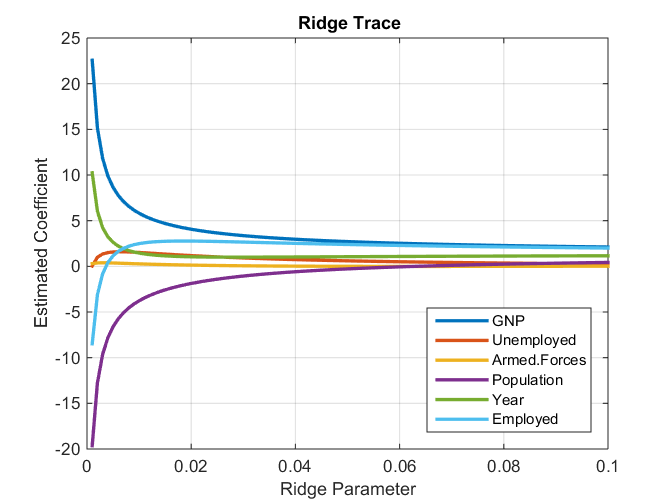
\includegraphics[width=.9\linewidth]{./images/ridge_trace.png}
\caption{\label{fig:org839b47e}Ridge Trace Example}
\end{figure}


\textbf{look for}
\begin{itemize}
\item spots where the line smooths out
\item where least change in \(b_k^r\) happens
\end{itemize}

finding \emph{c} is a bit of an art.

this formula can be used to convert standardized coefficients to unstandardized
coefficients.

\(b_k = (\frac{s_y}{s_k}) b_k^r\)

\(s_y\): standard dev of y
\(s_k\): standard error of \(b_k\)

\subsection{robust regression}
\label{sec:org94a0fff}
\begin{itemize}
\item reduce influential cases
\end{itemize}

uses \textbf{iteratively reweighted least squares} where \(w_i\) dampens influential
cases instead of heteroskedasticity.


\(u\): Scaled residual
0.345|4.685: tuning constants that are robust for 95\% of normal data.
Huber:

\begin{equation}
\begin{split}
w = \begin{cases}
1 & |u| \leq 1.345\\
\frac{1.345}{|u|} & |u| > 1.345
\end{cases}
\end{split}
\end{equation}

Bisquare:

\begin{equation}
\begin{split}
w = \begin{cases}
[1 - (\frac{u}{4.685})^2]^2 & |u| \leq 4.685\\
0 & |u| > 4.685
\end{cases}
\end{split}
\end{equation}

Huber is often used to obtain starting weights for Bisquare.

\subsubsection{\(u\)}
\label{sec:orgea83f6c}
\begin{itemize}
\item Semi-studentized residuals could be used but they are not resistant to
outliers
\item Mean Absolute Deviation (MAD) often used.

\(MAD = \frac{1}{0.6745} med (|e_i - med (e_i)|)\)

\(u_i = \frac{e_i}{MAD}\)

0.6745 is used to make this an unbiased estimate for \(\sigma\) from a normal distribution.
\end{itemize}

\subsection{Regression Tree (Non-parametric Method)}
\label{sec:org622825e}
\begin{itemize}
\item Split X's into distinct regions \emph{r} and run a regression on each region.
\item ``Growing a tree'' is finding the number of regions \emph{r} and the boundaries/split
points between them.
\item If the variance of the residuals in each region seem constant, splitting may
not be necessary.
\item The best split point minimizes \(SSE = \sum_{k = 1}^{r} SSE (R_{rk})\)
\item Once the optimal \emph{r} is chosen, each \emph{r} is subdivided to find the most
optimal SSE.
\item The chosen number of regions is done through validation studies, such as
choosing the tree that minimizes MSPR
\end{itemize}
\end{document}
